\documentclass[12pt]{article}
%DIF LATEXDIFF DIFFERENCE FILE


\usepackage[top=1in,left=1in, right = 1in, footskip=1in]{geometry}
\usepackage{url}
\usepackage{graphicx}
%\usepackage{adjustbox}

\usepackage{xcolor}
\usepackage{lineno}\renewcommand\thelinenumber{\color{gray}\arabic{linenumber}}
% \linenumbers

%DIF 11a11-14
\usepackage{pdflscape} %DIF > 
 %DIF > 
\usepackage{afterpage} %DIF > 
 %DIF > 
%DIF -------
\newcommand{\eref}[1]{Eq.~\ref{eq:#1}}
\newcommand{\fref}[1]{Fig.~\ref{fig:#1}}
\newcommand{\Fref}[1]{Fig.~\ref{fig:#1}}
\newcommand{\sref}[1]{Sec.~\ref{#1}}
\newcommand{\frange}[2]{Fig.~\ref{fig:#1}--\ref{fig:#2}}
\newcommand{\tref}[1]{Table~\ref{tab:#1}}
\newcommand{\tlab}[1]{\label{tab:#1}}
\newcommand{\seminar}{SE\mbox{$^m$}I\mbox{$^n$}R}

\usepackage{amsthm}
\usepackage{amsmath}
\usepackage{amssymb}
\usepackage{amsfonts}

%\usepackage{lineno}
%\linenumbers

\usepackage[pdfencoding=auto, psdextra]{hyperref}

\usepackage{natbib}
\bibliographystyle{chicago}
\date{\today}

\usepackage{xspace}
\newcommand*{\ie}{i.e.\@\xspace}

%DIF 37a41-43
\usepackage{array} %DIF > 
\newcolumntype{L}[1]{>{\raggedright\let\newline\\\arraybackslash\hspace{0pt}}m{#1}} %DIF > 
 %DIF > 
%DIF -------
\usepackage{color}

\usepackage{xspace}
\newcommand{\Rx}[1]{\ensuremath{{\mathcal R}_{#1}}\xspace}
% https://tex.stackexchange.com/questions/86565/drawbacks-of-xspace
% avoid double-\xspace
\newcommand{\Ro}{\ensuremath{{\mathcal R}_{0}}\xspace}
%DIF 44a51
\newcommand{\Rpool}{\ensuremath{{\mathcal R}_{\textrm{\tiny{pool}}}}\xspace} %DIF > 
%DIF -------
\newcommand{\RR}{\ensuremath{{\mathcal R}}}
\newcommand{\Rhat}{\ensuremath{{\hat\RR}}}
\newcommand{\tsub}[2]{#1_{{\textrm{\tiny #2}}}}

\newcommand{\comment}[3]{\textcolor{#1}{\textbf{[#2: }\textsl{#3}\textbf{]}}}

%DIF 50-51c58
%DIF < %% \newcommand{\rev}[1]{\comment{red}{REV}{#1}}
%DIF < \newcommand{\rev}[1]{}
%DIF -------
\newcommand{\rev}[1]{\comment{red}{REV}{#1}} %DIF > 
%DIF -------

\newcommand{\swp}[1]{\comment{magenta}{SWP}{#1}}
\newcommand{\jd}[1]{\comment{magenta}{JD}{#1}}
\newcommand{\djde}[1]{\comment{magenta}{DJDE}{#1}}
\newcommand{\bmb}[1]{\comment{magenta}{BMB}{#1}}
\newcommand{\dc}[1]{\comment{magenta}{DC}{#1}}
\newcommand{\jsw}[1]{\comment{magenta}{JSW}{#1}}
\newcommand{\mli}[1]{\comment{magenta}{MLi}{#1}}
\newcommand{\new}[1]{\textcolor{blue}{#1}}
%DIF PREAMBLE EXTENSION ADDED BY LATEXDIFF
%DIF UNDERLINE PREAMBLE %DIF PREAMBLE
\RequirePackage[normalem]{ulem} %DIF PREAMBLE
\RequirePackage{color}\definecolor{RED}{rgb}{1,0,0}\definecolor{BLUE}{rgb}{0,0,1} %DIF PREAMBLE
\providecommand{\DIFaddtex}[1]{{\protect\color{blue}\uwave{#1}}} %DIF PREAMBLE
\providecommand{\DIFdeltex}[1]{{\protect\color{red}\sout{#1}}}                      %DIF PREAMBLE
%DIF SAFE PREAMBLE %DIF PREAMBLE
\providecommand{\DIFaddbegin}{} %DIF PREAMBLE
\providecommand{\DIFaddend}{} %DIF PREAMBLE
\providecommand{\DIFdelbegin}{} %DIF PREAMBLE
\providecommand{\DIFdelend}{} %DIF PREAMBLE
%DIF FLOATSAFE PREAMBLE %DIF PREAMBLE
\providecommand{\DIFaddFL}[1]{\DIFadd{#1}} %DIF PREAMBLE
\providecommand{\DIFdelFL}[1]{\DIFdel{#1}} %DIF PREAMBLE
\providecommand{\DIFaddbeginFL}{} %DIF PREAMBLE
\providecommand{\DIFaddendFL}{} %DIF PREAMBLE
\providecommand{\DIFdelbeginFL}{} %DIF PREAMBLE
\providecommand{\DIFdelendFL}{} %DIF PREAMBLE
%DIF HYPERREF PREAMBLE %DIF PREAMBLE
\providecommand{\DIFadd}[1]{\texorpdfstring{\DIFaddtex{#1}}{#1}} %DIF PREAMBLE
\providecommand{\DIFdel}[1]{\texorpdfstring{\DIFdeltex{#1}}{}} %DIF PREAMBLE
\newcommand{\DIFscaledelfig}{0.5}
%DIF HIGHLIGHTGRAPHICS PREAMBLE %DIF PREAMBLE
\RequirePackage{settobox} %DIF PREAMBLE
\RequirePackage{letltxmacro} %DIF PREAMBLE
\newsavebox{\DIFdelgraphicsbox} %DIF PREAMBLE
\newlength{\DIFdelgraphicswidth} %DIF PREAMBLE
\newlength{\DIFdelgraphicsheight} %DIF PREAMBLE
% store original definition of \includegraphics %DIF PREAMBLE
\LetLtxMacro{\DIFOincludegraphics}{\includegraphics} %DIF PREAMBLE
\newcommand{\DIFaddincludegraphics}[2][]{{\color{blue}\fbox{\DIFOincludegraphics[#1]{#2}}}} %DIF PREAMBLE
\newcommand{\DIFdelincludegraphics}[2][]{% %DIF PREAMBLE
\sbox{\DIFdelgraphicsbox}{\DIFOincludegraphics[#1]{#2}}% %DIF PREAMBLE
\settoboxwidth{\DIFdelgraphicswidth}{\DIFdelgraphicsbox} %DIF PREAMBLE
\settoboxtotalheight{\DIFdelgraphicsheight}{\DIFdelgraphicsbox} %DIF PREAMBLE
\scalebox{\DIFscaledelfig}{% %DIF PREAMBLE
\parbox[b]{\DIFdelgraphicswidth}{\usebox{\DIFdelgraphicsbox}\\[-\baselineskip] \rule{\DIFdelgraphicswidth}{0em}}\llap{\resizebox{\DIFdelgraphicswidth}{\DIFdelgraphicsheight}{% %DIF PREAMBLE
\setlength{\unitlength}{\DIFdelgraphicswidth}% %DIF PREAMBLE
\begin{picture}(1,1)% %DIF PREAMBLE
\thicklines\linethickness{2pt} %DIF PREAMBLE
{\color[rgb]{1,0,0}\put(0,0){\framebox(1,1){}}}% %DIF PREAMBLE
{\color[rgb]{1,0,0}\put(0,0){\line( 1,1){1}}}% %DIF PREAMBLE
{\color[rgb]{1,0,0}\put(0,1){\line(1,-1){1}}}% %DIF PREAMBLE
\end{picture}% %DIF PREAMBLE
}\hspace*{3pt}}} %DIF PREAMBLE
} %DIF PREAMBLE
\LetLtxMacro{\DIFOaddbegin}{\DIFaddbegin} %DIF PREAMBLE
\LetLtxMacro{\DIFOaddend}{\DIFaddend} %DIF PREAMBLE
\LetLtxMacro{\DIFOdelbegin}{\DIFdelbegin} %DIF PREAMBLE
\LetLtxMacro{\DIFOdelend}{\DIFdelend} %DIF PREAMBLE
\DeclareRobustCommand{\DIFaddbegin}{\DIFOaddbegin \let\includegraphics\DIFaddincludegraphics} %DIF PREAMBLE
\DeclareRobustCommand{\DIFaddend}{\DIFOaddend \let\includegraphics\DIFOincludegraphics} %DIF PREAMBLE
\DeclareRobustCommand{\DIFdelbegin}{\DIFOdelbegin \let\includegraphics\DIFdelincludegraphics} %DIF PREAMBLE
\DeclareRobustCommand{\DIFdelend}{\DIFOaddend \let\includegraphics\DIFOincludegraphics} %DIF PREAMBLE
\LetLtxMacro{\DIFOaddbeginFL}{\DIFaddbeginFL} %DIF PREAMBLE
\LetLtxMacro{\DIFOaddendFL}{\DIFaddendFL} %DIF PREAMBLE
\LetLtxMacro{\DIFOdelbeginFL}{\DIFdelbeginFL} %DIF PREAMBLE
\LetLtxMacro{\DIFOdelendFL}{\DIFdelendFL} %DIF PREAMBLE
\DeclareRobustCommand{\DIFaddbeginFL}{\DIFOaddbeginFL \let\includegraphics\DIFaddincludegraphics} %DIF PREAMBLE
\DeclareRobustCommand{\DIFaddendFL}{\DIFOaddendFL \let\includegraphics\DIFOincludegraphics} %DIF PREAMBLE
\DeclareRobustCommand{\DIFdelbeginFL}{\DIFOdelbeginFL \let\includegraphics\DIFdelincludegraphics} %DIF PREAMBLE
\DeclareRobustCommand{\DIFdelendFL}{\DIFOaddendFL \let\includegraphics\DIFOincludegraphics} %DIF PREAMBLE
%DIF END PREAMBLE EXTENSION ADDED BY LATEXDIFF

\begin{document}

\begin{flushleft}{
	\Large
	\textbf\newline{
		Reconciling early-outbreak estimates of the basic reproductive number and its uncertainty: framework and applications to the novel coronavirus (SARS-CoV-2) outbreak
	}
}
\newline
\\
Sang Woo Park\textsuperscript{1,*}
Benjamin M.\ Bolker\textsuperscript{2,3,4}
David Champredon\textsuperscript{5}
David J.\,D.\ Earn\textsuperscript{3,4}
Michael Li\textsuperscript{2}
Joshua S.\ Weitz\textsuperscript{6, 7}
Bryan T.\ Grenfell\textsuperscript{1,8,9}
Jonathan Dushoff\textsuperscript{2,3,4,*}
\\
\bigskip
\textbf{1} Department of Ecology and Evolutionary Biology, Princeton University, Princeton, NJ, USA
\\
\textbf{2} Department of Biology, McMaster University, Hamilton, ON, Canada
\\
\textbf{3} Department of Mathematics and Statistics, McMaster University, Hamilton, ON, Canada
\\
\textbf{4} M.\,G.\,DeGroote Institute for Infectious Disease Research, McMaster University, Hamilton, ON, Canada
\\
\textbf{5} Department of Pathology and Laboratory Medicine, University of Western Ontario, London, Ontario, Canada
\\
\textbf{6} School of Biological Sciences, Georgia Institute of Technology, Atlanta, GA, USA
\\
\textbf{7} School of Physics, Georgia Institute of Technology, Atlanta, GA, USA
\\
\textbf{8} Division of International Epidemiology and Population Studies, Fogarty International Center, National Institutes of Health, Bethesda, MD, USA
\\
\textbf{9} Woodrow Wilson School of Public and International Affairs, Princeton University, Princeton, NJ, USA
\\
\bigskip

*Corresponding authors: swp2@princeton.edu and dushoff@mcmaster.ca
\end{flushleft}

\pagebreak

\section*{Abstract}
A novel coronavirus (SARS-CoV-2) \DIFdelbegin \DIFdel{has recently }\DIFdelend emerged as a global threat \DIFdelbegin \DIFdel{. 
}\DIFdelend \DIFaddbegin \DIFadd{in December 2019. 
}\DIFaddend As the epidemic progresses, \DIFdelbegin \DIFdel{many disease modelers have focused }\DIFdelend \DIFaddbegin \DIFadd{disease modelers continue to focus }\DIFaddend on estimating the basic reproductive number \Ro\DIFdelbegin \DIFdel{-- }\DIFdelend \DIFaddbegin \DIFadd{\ --- }\DIFaddend the average number of secondary cases caused by a primary case in an otherwise susceptible population.
The modeling approaches and resulting estimates of \Ro \DIFaddbegin \DIFadd{during the beginning of the outbreak }\DIFaddend vary widely, despite relying on similar data sources.
Here, we present a \DIFdelbegin \DIFdel{novel }\DIFdelend statistical framework for comparing and combining different estimates of \Ro across a wide range of models by decomposing the basic reproductive number into three key quantities: the exponential growth rate\DIFdelbegin \DIFdel{$r$}\DIFdelend , the mean generation interval\DIFdelbegin \DIFdel{$\bar G$}\DIFdelend , and the generation-interval dispersion\DIFdelbegin \DIFdel{$\kappa$.
We then }\DIFdelend \DIFaddbegin \DIFadd{.
We }\DIFaddend apply our framework to early estimates of \Ro for the SARS-CoV-2 outbreak\DIFdelbegin \DIFdel{.
We show that many early }\DIFdelend \DIFaddbegin \DIFadd{, showing that many }\DIFaddend \Ro estimates are overly confident.
Our results emphasize the importance of propagating uncertainties in all components of \Ro, including the shape of the generation-interval distribution, in efforts to estimate \Ro at the outset of an epidemic.

\section*{Keywords}

SARS-CoV-2, COVID-19, novel coronavirus, basic reproductive number, generation interval, Bayesian multilevel model

\section{Introduction}

Since December 2019, a novel coronavirus (SARS-CoV-2) has been spreading \DIFdelbegin \DIFdel{in China and other parts of the world }\DIFdelend \DIFaddbegin \DIFadd{globally }\DIFaddend \citep{pneumonia}.
Although the virus is \DIFdelbegin \DIFdel{believed }\DIFdelend \DIFaddbegin \DIFadd{likely }\DIFaddend to have originated from animal \DIFdelbegin \DIFdel{reservoirs \mbox{%DIFAUXCMD
\citep{cdcncov}}\hspace{0pt}%DIFAUXCMD
}\DIFdelend \DIFaddbegin \DIFadd{hosts \mbox{%DIFAUXCMD
\citep{andersen2020proximal}}\hspace{0pt}%DIFAUXCMD
}\DIFaddend , the ability of SARS-CoV-2 \DIFdelbegin \DIFdel{ability }\DIFdelend to directly transmit between humans\DIFaddbegin \DIFadd{, particularly without symptoms, }\DIFaddend has posed a greater threat for its spread \DIFdelbegin \DIFdel{\mbox{%DIFAUXCMD
\citep{huang2020clinical,who26report}}\hspace{0pt}%DIFAUXCMD
}\DIFdelend \DIFaddbegin \DIFadd{\mbox{%DIFAUXCMD
\citep{he2020temporal}}\hspace{0pt}%DIFAUXCMD
}\DIFaddend .
As of \DIFdelbegin \DIFdel{February 27}\DIFdelend \DIFaddbegin \DIFadd{May 11}\DIFaddend , 2020, \DIFdelbegin \DIFdel{the World Health Organization (WHO) has confirmed 82,294 }\DIFdelend \DIFaddbegin \DIFadd{more than 4 million }\DIFaddend cases of the coronavirus disease \DIFaddbegin \DIFadd{2019 }\DIFaddend (COVID-19) \DIFdelbegin \DIFdel{, including 3,664 confirmed cases in 46 different countries, outside China \mbox{%DIFAUXCMD
\citep{who38report}}\hspace{0pt}%DIFAUXCMD
.
%DIF <  Also on January 30, 2020, WHO declared the outbreak a Public Health Emergency of International Concern \citep{whoemer}.
}\DIFdelend \DIFaddbegin \DIFadd{have been confirmed internationally \mbox{%DIFAUXCMD
\citep{who112}}\hspace{0pt}%DIFAUXCMD
.
}\DIFaddend 

As \DIFdelbegin \DIFdel{the disease continues to spread , many researchers have already published their }\DIFdelend \DIFaddbegin \DIFadd{SARS-CoV-2 began to spread in parts of China outside Hubei province, as well as in other countries, many }\DIFaddend analyses of the outbreak \DIFaddbegin \DIFadd{were published }\DIFaddend as pre-prints \DIFdelbegin \DIFdel{(e.g., \mbox{%DIFAUXCMD
\cite{bedfordncov, imaincov, liuncov, majumderncov, readncov, zhaoncov}}\hspace{0pt}%DIFAUXCMD
) }\DIFdelend \DIFaddbegin \DIFadd{\mbox{%DIFAUXCMD
\citep{bedfordncov, imaincov, liuncov, majumderncov, readncov, zhaoncov} }\hspace{0pt}%DIFAUXCMD
}\DIFaddend and in peer-reviewed journals \DIFdelbegin \DIFdel{(e.
g., \mbox{%DIFAUXCMD
\cite{li2020early, riou2020pattern, wu2020nowcasting, zhao2020preliminary}}\hspace{0pt}%DIFAUXCMD
), focusing in particular on estimates of }\DIFdelend \DIFaddbegin \DIFadd{\mbox{%DIFAUXCMD
\citep{li2020early, riou2020pattern, wu2020nowcasting, zhao2020preliminary}}\hspace{0pt}%DIFAUXCMD
.
These analyses focused on estimating }\DIFaddend the basic reproductive number \Ro\DIFdelbegin \DIFdel{(i.e., }\DIFdelend \DIFaddbegin \DIFadd{\ --- }\DIFaddend the average number of secondary cases generated by a primary case in a fully susceptible population \citep{anderson1991infectious, diekmann1990definition} \DIFdelbegin \DIFdel{).
Estimates of the basic reproductive number are of interest during an outbreak because they provide information about the level of intervention required to interrupt transmission \mbox{%DIFAUXCMD
\citep{anderson1991infectious}}\hspace{0pt}%DIFAUXCMD
, and about the potential final size of the outbreak \mbox{%DIFAUXCMD
\citep{anderson1991infectious, ma2006generality}}\hspace{0pt}%DIFAUXCMD
.
}\DIFdelend \DIFaddbegin \DIFadd{--- in order to assess the pandemic potential of SARS-CoV-2.
Rapid dissemination of these early analyses played an important role in shaping the response to the outbreak \mbox{%DIFAUXCMD
\citep{majumder2020early}}\hspace{0pt}%DIFAUXCMD
.
}

\DIFaddend We commend these researchers for their timely contribution and those who made the data publicly available.
However, \DIFdelbegin \DIFdel{it can be difficult to compare a disparate set of }\DIFdelend \DIFaddbegin \DIFadd{the }\DIFaddend estimates of \Ro from different research groups (as well as the associated degrees of uncertainty) \DIFaddbegin \DIFadd{vary considerably even though most analyses rely on similar data --- reports of confirmed cases from China, particularly from Wuhan City.
Comparing a disparate set of estimates of }\Ro \DIFadd{can be difficult }\DIFaddend when the estimation methods and their underlying assumptions vary widely.
\DIFaddbegin \DIFadd{In some cases, similar methods can give different estimates; in other cases, different methods can give similar estimates.
Understanding the differences between }\Ro \DIFadd{estimates is critical to controlling an epidemic as }\Ro \DIFadd{provides information about the level of intervention required to prevent further transmission \mbox{%DIFAUXCMD
\citep{anderson1991infectious}}\hspace{0pt}%DIFAUXCMD
, and about the potential final size of the outbreak \mbox{%DIFAUXCMD
\citep{anderson1991infectious, ma2006generality}}\hspace{0pt}%DIFAUXCMD
.
}\DIFaddend 

Here, we show that a wide range of approaches to estimating \Ro can be understood and compared in terms of estimates of three quantities: the exponential growth rate $r$, the mean generation interval $\bar G$, and the generation-interval dispersion $\kappa$.
The generation interval, defined as the interval between the time when an individual becomes infected and the time when that individual infects another individual \citep{svensson2007note}, \DIFdelbegin \DIFdel{plays a key role in shaping }\DIFdelend \DIFaddbegin \DIFadd{characterizes }\DIFaddend the relationship between $r$ and \Ro \citep{wearing2005appropriate, roberts2007model, wallinga2007generation, park2019practical};
therefore, estimates of \Ro \DIFdelbegin \DIFdel{from different models directly depend on their implicit }\DIFdelend \DIFaddbegin \DIFadd{depend directly on their }\DIFaddend assumptions about the generation-interval distribution and the exponential growth rate.
Early in an epidemic, information is scarce and there is \DIFdelbegin \DIFdel{inevitably a great deal of }\DIFdelend uncertainty surrounding both case reports (affecting the estimates of the exponential growth rate) and contact tracing (affecting the estimates of the generation-interval distribution).
\DIFdelbegin \DIFdel{We suggest that disease modelers should make sure their assumptions about these three quantities are clear and reasonable, and that estimates of uncertainty in }\DIFdelend \DIFaddbegin \DIFadd{Ignoring these uncertainties leads to overly confident conclusions.
}

\DIFadd{To formalize the estimation of uncertainty at the onset of an outbreak, we present a statistical framework for averaging across estimates of basic reproductive number }\DIFaddend \Ro \DIFdelbegin \DIFdel{should propagate error from all three sources \mbox{%DIFAUXCMD
\citep{elderd2006uncertainty}}\hspace{0pt}%DIFAUXCMD
. 
}%DIFDELCMD < 

%DIFDELCMD < %%%
\DIFdel{We compare }\DIFdelend \DIFaddbegin \DIFadd{from multiple studies. 
We apply the method to }\DIFaddend seven disparate models published online \DIFaddbegin \DIFadd{as pre-prints }\DIFaddend between January 23--26, 2020 that \DIFdelbegin \DIFdel{estimated }\DIFdelend \DIFaddbegin \DIFadd{estimate }\DIFaddend \Ro for the SARS-CoV-2 outbreak \DIFaddbegin \DIFadd{in Wuhan City, China }\DIFaddend \citep{bedfordncov, imaincov, liuncov, majumderncov, readncov, riouncov, zhaoncov}.
\DIFdelbegin \DIFdel{We use a Bayesian multilevel model to construct pooled estimates for the }\DIFdelend \DIFaddbegin \DIFadd{Previous studies have directly calculated the average of reported }\Ro \DIFadd{values \mbox{%DIFAUXCMD
\citep{majumder2020early, liu2020reproductive} }\hspace{0pt}%DIFAUXCMD
but such methods mask differences in underlying model assumptions and statistical methods.
Instead, we decompose estimated }\Ro \DIFadd{into }\DIFaddend three key quantities \DIFdelbegin \DIFdel{: }\DIFdelend \DIFaddbegin \DIFadd{(}\DIFaddend $r$, $\bar G$, and $\kappa$\DIFdelbegin \DIFdel{;
the pooled estimates reflect the }\DIFdelend \DIFaddbegin \DIFadd{) and calculate the average (pooled estimates) of these key parameters.
Calculating }\Ro \DIFadd{based on the pooled estimates allows us to average appropriately across the }\DIFaddend uncertainties present in modeling approaches and \DIFaddbegin \DIFadd{in }\DIFaddend their underlying assumptions.
We use these pooled estimates to illustrate the importance of propagating different sources of error, particularly uncertainty in both the growth rate and the generation interval.
\DIFdelbegin \DIFdel{We also use our framework to tease apart which assumptions of these different models led to their different estimates and confidence intervals.
Despite the availability of more recent and/or updated estimates of }%DIFDELCMD < \Ro%%%
\DIFdel{, we restrict ourselves to the estimates above in order to focus on the resolution of uncertainty in the earliest stages of an epidemic.
}\DIFdelend 

\section{Methods}

\subsection{Description of the studies}

\DIFdelbegin %DIFDELCMD < \begin{table}[t]
%DIFDELCMD < \begin{center}
%DIFDELCMD < \scriptsize
%DIFDELCMD < \begin{tabular}{l|p{3.5cm}|p{2.5cm}|p{2.7cm}|l}
%DIFDELCMD <  & %%%
\DIFdelFL{Basic reproductive}%DIFDELCMD < \newline %%%
\DIFdelFL{number }%DIFDELCMD < \Ro & %%%
\DIFdelFL{Mean generation}%DIFDELCMD < \newline %%%
\DIFdelFL{interval $\bar G$ (days) }%DIFDELCMD < & %%%
\DIFdelFL{Generation-interval}%DIFDELCMD < \newline %%%
\DIFdelFL{dispersion $\kappa$ }%DIFDELCMD < & \\
%DIFDELCMD < \hline
%DIFDELCMD < %%%
\DIFdelFL{Study 1 }%DIFDELCMD < & %%%
\DIFdelFL{1.5--3.5 }%DIFDELCMD < & %%%
\DIFdelFL{10 }%DIFDELCMD < & %%%
\DIFdelFL{1 }%DIFDELCMD < & %%%
\DIFdelFL{\mbox{%DIFAUXCMD
\cite{bedfordncov} }\hspace{0pt}%DIFAUXCMD
}%DIFDELCMD < \\
%DIFDELCMD < \hline
%DIFDELCMD < %%%
\DIFdelFL{Study 2 }%DIFDELCMD < & %%%
\DIFdelFL{2.5 (1.5--3.5)$^\ast$ }%DIFDELCMD < & %%%
\DIFdelFL{8.4 }%DIFDELCMD < & %%%
\DIFdelFL{unspecified$^\dagger$ }%DIFDELCMD < & %%%
\DIFdelFL{\mbox{%DIFAUXCMD
\cite{imaincov} }\hspace{0pt}%DIFAUXCMD
}%DIFDELCMD < \\
%DIFDELCMD < \hline
%DIFDELCMD < %%%
\DIFdelFL{Study 3 }%DIFDELCMD < & %%%
\DIFdelFL{2.92 (95\% CI: 2.28--3.67) }%DIFDELCMD < & %%%
\DIFdelFL{8.4 }%DIFDELCMD < & %%%
\DIFdelFL{0.2 }%DIFDELCMD < & %%%
\DIFdelFL{\mbox{%DIFAUXCMD
\cite{liuncov} }\hspace{0pt}%DIFAUXCMD
}%DIFDELCMD < \\
%DIFDELCMD < \hline
%DIFDELCMD < %%%
\DIFdelFL{Study 4 }%DIFDELCMD < & %%%
\DIFdelFL{3.8 (95\% CI: 3.6--4.0) }%DIFDELCMD < & %%%
\DIFdelFL{7.6 }%DIFDELCMD < & %%%
\DIFdelFL{0.5 }%DIFDELCMD < & %%%
\DIFdelFL{\mbox{%DIFAUXCMD
\cite{readncov} }\hspace{0pt}%DIFAUXCMD
}%DIFDELCMD < \\
%DIFDELCMD < \hline
%DIFDELCMD < %%%
\DIFdelFL{Study 5 }%DIFDELCMD < & %%%
\DIFdelFL{2.2 (90\% CI: 1.4--3.8) }%DIFDELCMD < & %%%
\DIFdelFL{7--14 }%DIFDELCMD < & %%%
\DIFdelFL{0.5 }%DIFDELCMD < & %%%
\DIFdelFL{\mbox{%DIFAUXCMD
\cite{riouncov} }\hspace{0pt}%DIFAUXCMD
}%DIFDELCMD < \\
%DIFDELCMD < \hline
%DIFDELCMD < %%%
\DIFdelFL{Study 6 }%DIFDELCMD < & %%%
\DIFdelFL{5.47 (95\% CI: 4.16--7.10)$^\ddagger$ }%DIFDELCMD < & %%%
\DIFdelFL{7.6--8.4 }%DIFDELCMD < & %%%
\DIFdelFL{0.2 }%DIFDELCMD < & %%%
\DIFdelFL{\mbox{%DIFAUXCMD
\cite{zhaoncov} }\hspace{0pt}%DIFAUXCMD
}%DIFDELCMD < \\
%DIFDELCMD < \hline
%DIFDELCMD < %%%
\DIFdelFL{Study 7 }%DIFDELCMD < & %%%
\DIFdelFL{2.0--3.1 }%DIFDELCMD < & %%%
\DIFdelFL{6--10 }%DIFDELCMD < & %%%
\DIFdelFL{0 }%DIFDELCMD < & %%%
\DIFdelFL{\mbox{%DIFAUXCMD
\cite{majumderncov} }\hspace{0pt}%DIFAUXCMD
}%DIFDELCMD < \\
%DIFDELCMD < \hline
%DIFDELCMD < \end{tabular}
%DIFDELCMD < \end{center}
%DIFDELCMD < %%%
%DIFDELCMD < \caption{%
{%DIFAUXCMD
\textbf{\DIFdelFL{Reported estimates of the basic reproductive number and the assumptions about the generation-interval distributions.}}
%DIFAUXCMD
\DIFdelFL{Estimates of }%DIFDELCMD < \Ro %%%
\DIFdelFL{and their assumptions about the shape of the generation interval distributions were collected from 7 studies.
$^\ast$We treat these intervals as a 95\% confidence interval in our analysis.
$^\dagger$We assume $\kappa = 0.5$ in our analysis.
$^\ddagger$The authors presented }%DIFDELCMD < \Ro %%%
\DIFdelFL{estimates under different assumptions regarding the reporting rate; we use their baseline scenario in our analysis to remain consistent with other studies, which do not account for changes in the reporting rate.
}}
%DIFAUXCMD
%DIFDELCMD < \end{table}
%DIFDELCMD < %%%
\DIFdelend \DIFaddbegin \afterpage{%
\clearpage
    \begin{landscape}
\begin{table}[!th]
\begin{center}
\scriptsize
\begin{tabular}{l|L{2cm}|L{3.2cm}|L{2.8cm}|L{2.5cm}|L{2.4cm}|L{2.7cm}|L{2cm}}
 & Model & Data (study period) & Data source & Basic reproductive\newline number \Ro & Mean generation\newline interval $\bar G$ (days) & Generation-interval\newline dispersion $\kappa$ & Reference \\
\hline
Study 1 & Deterministic branching process model & Total number of cases in Wuhan City, China\newline (Jan 18, 2020) & Estimated by \cite{imaincov0} & 1.5--3.5 & 10 & 1 & \cite{bedfordncov} \\
\hline
Study 2 & Stochastic branching process model & Total number of cases in Wuhan City, China\newline (Jan 18, 2020) & Estimated by \cite{imaincov0}  & 2.6 (1.5--3.5)$^\ast$ & 8.4 & Not reported$^\dagger$ & \cite{imaincov} \\
\hline
Study 3 & Poisson offspring distribution model & Confirmed cases from China and other countries\newline (Dec 29, 2019--Jan 23, 2020) & Medical records and epidemiological investigations from Guangdong Province, China, and official websites of other regions in China & 2.92 (95\% CI: 2.28--3.67) & 8.4 & 0.2 & \cite{liuncov} \\
\hline
Study 4 & Deterministic Metapopulation Susceptible-Exposed-Infected-Recovered (SEIR) model & Confirmed cases from China and other countries\newline (Jan 1--21, 2020) & Not reported & 3.8 (95\% CI: 3.6--4.0) & 7.6 & 0.5 & \cite{readncov} \\
\hline
Study 5 & Stochastic branching process model & Total number of cases in Wuhan City, China\newline (Jan 18, 2020) & Estimated by \cite{imaincov0} & 2.2 (90\% CI: 1.4--3.8) & 7--14 & 0.5 & \cite{riouncov} \\
\hline
Study 6 & Exponential growth model & Confirmed cases from China\newline (Jan 10--22, 2020) & Wuhan
Municipal Health Commission, China and National Health Commission of China & 5.47 (95\% CI: 4.16--7.10)$^\ddagger$ & 7.6--8.4 & 0.2 & \cite{zhaoncov} \\
\hline
Study 7 & Incidence Decay and Exponential Adjustment (IDEA) model & Reported cases from Wuhan City, China\newline (Dec 1, 2019--Jan 26, 2020) & World	Health Organization, National Health Commission of China, Wuhan Municipal	Health Commission, and \cite{huang2020clinical} & 2.0--3.1 & 6--10 & 0 & \cite{majumderncov} \\
\hline
\end{tabular}
\end{center}
\caption{
\textbf{Summary of the models, analyzed data, reported estimates of the basic reproductive number, and the assumptions about the generation-interval distributions.}
Model details, estimates of \Ro, and their assumptions about the shape of the generation interval distributions were collected from 7 studies.
Generation-interval dispersion represent the squared coefficients of variation in generation intervals.
$^\ast$These intervals reflect \Ro values for best and worst scenarios. We treat these intervals as a 90\% credible interval in our analysis.
$^\dagger$We assume $\kappa = 0.5$ in our analysis.
$^\ddagger$The authors presented \Ro estimates under different assumptions regarding the reporting rate; we use their baseline scenario in our analysis to remain consistent with other studies, which do not account for changes in the reporting rate.
}
\end{table}
\end{landscape}
\clearpage
}
\DIFaddend 

We gathered information on estimates of \Ro \DIFdelbegin \DIFdel{and their assumptions about the underlying generation-interval distributions from 7 }\DIFdelend \DIFaddbegin \DIFadd{for the SARS-CoV-2 outbreak in Wuhan City, China and their model assumptions from seven }\DIFaddend articles that were published online between January 23--26, \DIFdelbegin \DIFdel{2020 (Table 1).
}\DIFdelend \DIFaddbegin \DIFadd{2020.
}\DIFaddend Five studies \citep{liuncov, majumderncov, readncov, riouncov, zhaoncov} were uploaded to pre-print servers (bioRxiv, medRxiv, and SSRN); one report was posted on the \DIFdelbegin \DIFdel{web site }\DIFdelend \DIFaddbegin \DIFadd{website }\DIFaddend of Imperial College London \citep{imaincov}; and one report was posted on \DIFdelbegin \DIFdel{nextstrain.org \mbox{%DIFAUXCMD
\citep{bedfordncov} }\hspace{0pt}%DIFAUXCMD
.
Their modeling approaches vary widely: a branching process model \mbox{%DIFAUXCMD
\citep{bedfordncov, imaincov, riouncov}}\hspace{0pt}%DIFAUXCMD
, a deterministic Susceptible-Exposed-Infected-Recovered (SEIR) model \mbox{%DIFAUXCMD
\citep{readncov}}\hspace{0pt}%DIFAUXCMD
, an exponential growth model \mbox{%DIFAUXCMD
\citep{zhaoncov}}\hspace{0pt}%DIFAUXCMD
, a Poisson offspring distribution model \mbox{%DIFAUXCMD
\citep{liuncov}}\hspace{0pt}%DIFAUXCMD
, }\DIFdelend \DIFaddbegin \url{nextstrain.org} \DIFadd{\mbox{%DIFAUXCMD
\citep{bedfordncov} }\hspace{0pt}%DIFAUXCMD
(Table 1).
}

\subsection{\DIFadd{Model assumptions}}

\DIFadd{Despite a wide range of models considered across Study 1--7, all of them assume that the epidemic initially grows exponentially.
The IDEA model (used in Study 7) includes a discount parameter $d$ that allows the model to deviate from exponential growth when $d \neq 0$ \mbox{%DIFAUXCMD
\citep{fisman2013idea}}\hspace{0pt}%DIFAUXCMD
, but Study 7 estimates $d=0$ across all parameters they consider.
Even though some studies consider reported cases up to January 26, 2020 --- three days after the travel restriction that took place on January 23, 2020 \mbox{%DIFAUXCMD
\citep{Tianeabb6105} }\hspace{0pt}%DIFAUXCMD
--- the exponential growth assumption can still describe the number of reported cases reasonably well;
given the incubation period of around 5 days \mbox{%DIFAUXCMD
\citep{lauer2020incubation} }\hspace{0pt}%DIFAUXCMD
as well as reporting delays of around 5 days \mbox{%DIFAUXCMD
\citep{sun2020early}}\hspace{0pt}%DIFAUXCMD
, the majority of reported cases during the study periods are likely to have been infected prior to the travel ban.
}

\DIFadd{When the epidemic is growing exponentially, the estimated basic reproductive number is determined by the exponential growth rate $r$ and the intrinsic generation-interval distribution $g(\tau)$, which describes the infection time of secondary cases caused by a primary case in a fully susceptible population \mbox{%DIFAUXCMD
\citep{champredon2015intrinsic}}\hspace{0pt}%DIFAUXCMD
, via the Euler-Lotka equation \mbox{%DIFAUXCMD
\citep{wallinga2007generation}}\hspace{0pt}%DIFAUXCMD
:
}\begin{linenomath*}
\begin{equation}
\DIFadd{\frac{1}{\Ro} = \int \exp(-r\tau) g(\tau) \, d\tau.
\label{eq:euler}
}\end{equation}
\end{linenomath*}
\DIFadd{Therefore, it is sufficient to consider the estimates and assumptions about the exponential growth rates and the shapes of the generation-interval distributions to understand disparate estimates of the basic reproductive number.
All model assumptions reduce to properties of the exponential growth rate $r$ and the shape of the generation-interval distribution $g(\tau)$.
For example, if a model relies on overly confident assumptions about the underlying observation (how new cases are reported) or process (how new cases are generated) model, the estimated confidence or credible intervals associated with the exponential growth rates or parameters of the generation-interval distributions will necessarily be narrow.
}

\DIFadd{As most studies do not report their estimates of the exponential growth rate, we first summarize model outcomes using reported (either estimated or assumed) values of the basic reproductive number }\Ro\DIFadd{, mean generation interval $\bar G$ }\DIFaddend and \DIFaddbegin \DIFadd{generation-interval dispersion $\kappa$, represented by the squared coefficient of variation (Table 1) ---
we re-estimate the corresponding exponential growth rates from these values later.
Study 2 only reports their assumptions about the mean generation interval; for simplicity, we assume $\kappa = 0.5$ in our analysis.
Study 6 presents }\Ro \DIFadd{estimates under 12 different scenarios regarding reporting rates (0, 0.5, 1 or 2 fold increase in reporting rate) and the shapes of }\DIFaddend the \DIFdelbegin \DIFdel{Incidence Decay and Exponential Adjustment (IDEA) model \mbox{%DIFAUXCMD
\citep{majumderncov}}\hspace{0pt}%DIFAUXCMD
.
Four studies estimated }\DIFdelend \DIFaddbegin \DIFadd{generation-interval distributions based on previous coronavirus outbreaks (Middle East Respiratory Syndrome, MERS; Severe Acute Respiratory Syndrome, SARS; and their average) ---
we use their baseline scenario in our analysis to remain consistent with other studies, which do not account for changes in the reporting rate.
While estimates of }\DIFaddend \Ro \DIFdelbegin \DIFdel{by directly fitting their models to incidence data \mbox{%DIFAUXCMD
\citep{readncov, zhaoncov, liuncov, majumderncov}}\hspace{0pt}%DIFAUXCMD
.
The remaining three studies estimated }\DIFdelend \DIFaddbegin \DIFadd{and the associated confidence intervals for Study 6 in Table 1 are based on $\bar G = 8\,\mathrm{days}$, we account for the uncertainty they consider for $\bar G$ in our formal analysis.
}

\DIFadd{While most studies report confidence or credible intervals to quantify uncertainties associated with their estimates, some use different measures.
In particular, Study 2 reports a range of }\DIFaddend \Ro \DIFdelbegin \DIFdel{by comparing the predicted number of cases from their models with the estimated number of total }\DIFdelend \DIFaddbegin \DIFadd{for the worst and best case scenarios, which correspond to the values of }\Ro \DIFadd{such that 95\% and 5\% of the simulated total number of }\DIFaddend cases by January 18\DIFdelbegin \DIFdel{(between 1, 000 and 9, 7000 \mbox{%DIFAUXCMD
\citep{imaincov0}}\hspace{0pt}%DIFAUXCMD
)
}\DIFdelend \DIFaddbegin \DIFadd{, 2020 are greater than or equal to 4000, respectively;
for simplicity, we treat these intervals as a 90\% credible interval in our analysis.
Uncertainty ranges reported by Study 1 and Study 7 are assumed to be uniform ranges.
}

\DIFaddend Some of these studies have now been published in peer-reviewed journals \citep{riou2020pattern, zhao2020preliminary} or have been updated with better uncertainty quantification \citep{readncov2}.
\DIFdelbegin %DIFDELCMD < 

%DIFDELCMD < %%%
\subsection{\DIFdel{Gamma approximation framework for linking $r$ and $\Ro$}}
%DIFAUXCMD
\addtocounter{subsection}{-1}%DIFAUXCMD
%DIFDELCMD < 

%DIFDELCMD < %%%
\DIFdel{Early in an outbreak, }%DIFDELCMD < \Ro %%%
\DIFdel{is difficult to estimate directly;
instead, }%DIFDELCMD < \Ro %%%
\DIFdel{is often inferred from the exponential growth rate $r$, which can be estimated reliably from incidence data \mbox{%DIFAUXCMD
\citep{ma2014estimating}}\hspace{0pt}%DIFAUXCMD
.
Given an estimate of the exponential growth rate $r$ and an }\emph{\DIFdel{intrinsic}} %DIFAUXCMD
\DIFdel{generation-interval distribution $g(\tau)$ \mbox{%DIFAUXCMD
\citep{champredon2015intrinsic}}\hspace{0pt}%DIFAUXCMD
, the basic reproductive
number can be estimated via the Euler-Lotka equation \mbox{%DIFAUXCMD
\citep{wallinga2007generation}}\hspace{0pt}%DIFAUXCMD
:
}%DIFDELCMD < \begin{linenomath*}
%DIFDELCMD < %%%
\begin{displaymath}
\DIFdel{1/\Ro = \int \exp(-r\tau) g(\tau) \, d\tau.
%DIFDELCMD < \label{eq:euler}%%%
}\end{displaymath}%DIFAUXCMD
%DIFDELCMD < \end{linenomath*}
%DIFDELCMD < %%%
\DIFdel{In other words, }\DIFdelend \DIFaddbegin \DIFadd{As our primary focus is on the resolution of uncertainty in the available information during the earliest stages of an epidemic, rather than to provide more precise or accurate }\DIFaddend estimates of \Ro\DIFdelbegin \DIFdel{must
depend on the assumptions about the
exponential growth rate $r$ and the shape of the generation-interval distribution $g(\tau)$.
}\DIFdelend \DIFaddbegin \DIFadd{, we focus strictly on estimates that were published between January 23--26, 2020.
}\DIFaddend 

\DIFaddbegin \subsection{\DIFadd{Gamma approximation framework for linking $r$ and $\Ro$}}

\DIFaddend Here, we use the gamma approximation framework \DIFdelbegin \DIFdel{\mbox{%DIFAUXCMD
\citep{park2019practical} }\hspace{0pt}%DIFAUXCMD
to }\DIFdelend \DIFaddbegin \DIFadd{to the generation-interval distribution \mbox{%DIFAUXCMD
\citep{nishiura2009transmission, mcbryde2009early, roberts2011early, trichereau2012estimation, nishiura2015theoretical, park2019practical} }\hspace{0pt}%DIFAUXCMD
to }\DIFaddend (i) characterize the amount of uncertainty present in the exponential growth rates and the shape of the generation-interval distribution and (ii) assess the degree to which these uncertainties affect the estimate of \Ro.
\DIFaddbegin \DIFadd{The gamma distribution provides a reasonable approximation for generation-interval distributions of many diseases, including Ebola, measles, and rabies \mbox{%DIFAUXCMD
\citep{park2019practical}}\hspace{0pt}%DIFAUXCMD
.
Studies 1, 5, 6, and 7 also used a gamma distribution (including the special cases of Dirac delta and exponential distributions) to model the generation-interval distribution for SARS-CoV-2.
}\DIFaddend Assuming that generation intervals follow a gamma distribution with \DIFdelbegin \DIFdel{the mean }\DIFdelend \DIFaddbegin \DIFadd{mean generation interval }\DIFaddend $\bar G$ and \DIFaddbegin \DIFadd{generation-interval dispersion $\kappa$, represented by }\DIFaddend the squared coefficient of variation \DIFdelbegin \DIFdel{$\kappa$}\DIFdelend \DIFaddbegin \DIFadd{of a gamma distribution}\DIFaddend , we have \DIFaddbegin \DIFadd{\mbox{%DIFAUXCMD
\citep{park2019practical}}\hspace{0pt}%DIFAUXCMD
:
}\DIFaddend \begin{linenomath*}
\begin{equation}
\Ro = \left(1 + \kappa r \bar{G}\right)^{1/\kappa}.
\label{eq:gamma}
\end{equation}
\end{linenomath*}
This equation demonstrates that a generation-interval distribution that has a larger mean (higher $\bar{G}$) or is less variable (lower $\kappa$) \DIFdelbegin \DIFdel{will give }\DIFdelend \DIFaddbegin \DIFadd{gives }\DIFaddend a higher estimate of \Ro for the same value of $r$ \citep{wallinga2007generation}.

\subsection{\DIFdelbegin \DIFdel{Statistical framework}\DIFdelend \DIFaddbegin \DIFadd{Re-estimation of the exponential growth rate}\DIFaddend }

As most studies do not report their estimates of the exponential growth rate, we first \DIFdelbegin \DIFdel{recalculate }\DIFdelend \DIFaddbegin \DIFadd{re-estimate }\DIFaddend the exponential growth rate that \DIFdelbegin \DIFdel{correspond }\DIFdelend \DIFaddbegin \DIFadd{corresponds }\DIFaddend to their model assumptions.
\DIFdelbegin \DIFdel{We do so by modeling reported distributionsof the }\DIFdelend \DIFaddbegin \DIFadd{Since the estimates of the basic reproductive number }\Ro \DIFadd{is determined by the exponential growth rate and the shape of generation-interval distributions, we can calculate the exponential growth rate from the basic reproductive number }\Ro\DIFadd{, the mean generation interval $\bar G$, and the generation-interval dispersion $\kappa$.
First, to account for uncertainties in these parameters, we model reported values of the basic }\DIFaddend reproductive number \Ro, the mean generation interval $\bar G$, and the generation-interval dispersion \DIFdelbegin \DIFdel{parameter }\DIFdelend $\kappa$ with appropriate probability distributions\DIFdelbegin \DIFdel{;
we used }\DIFdelend \DIFaddbegin \DIFadd{.
We use }\DIFaddend gamma distributions to model values reported with confidence \DIFdelbegin \DIFdel{intervals }\DIFdelend \DIFaddbegin \DIFadd{or credible intervals (CI) }\DIFaddend and uniform distributions to model values reported with ranges\DIFdelbegin \DIFdel{.
}\DIFdelend \DIFaddbegin \DIFadd{;
when confidence or credible intervals are reported, we parameterize the gamma distribution such that (i) its mean matches the estimated value and (ii) the probability that a random variable following the specified gamma distribution falls between the lower and upper confidence or credible limits is equal to the reported confidence or credible level. 
This probability does not need to be calculated from equi-tailed quantiles.
}\DIFaddend For example, Study 3 estimated $\Ro = 2.92$ (95\% CI: 2.28--3.67);
we model this estimate as a gamma distribution with a mean of 2.92 and a shape parameter of 67, which has a 95\% probability of containing a value between 2.28 and 3.67 (see Table 2 for a complete description).
\DIFaddbegin 

\DIFaddend For each study $i$, we construct a family of parameter sets by drawing \DIFdelbegin \DIFdel{100,000 }\DIFdelend \DIFaddbegin \DIFadd{$10^5$ }\DIFaddend random samples from the \DIFaddbegin \DIFadd{corresponding }\DIFaddend probability distributions (Table 2) that represent the estimates of \DIFdelbegin %DIFDELCMD < \Rx{0i} %%%
\DIFdelend \DIFaddbegin \DIFadd{$(\Ro)_{i,m}$ }\DIFaddend and the assumed values of \DIFdelbegin \DIFdel{$\bar G_i$ and $\kappa_i$ }\DIFdelend \DIFaddbegin \DIFadd{$\bar G_{i,m}$ and $\kappa_{i,m}$ }\DIFaddend and calculate the exponential growth rate \DIFdelbegin \DIFdel{$r_i$ via the inverse of }\DIFdelend \DIFaddbegin \DIFadd{$r_{i,m}$ by inverting }\DIFaddend \eref{gamma}:
\begin{linenomath*}
\begin{equation}
r\DIFdelbegin \DIFdel{_i }\DIFdelend \DIFaddbegin \DIFadd{_{i,m} }\DIFaddend = \DIFdelbegin \DIFdel{\frac{\Rx{0i}^{\kappa_i} - 1}{\kappa_i \bar{G}_i}.
}\DIFdelend \DIFaddbegin \DIFadd{\frac{\left[(\Ro)_{i,m}\right]^{\kappa_{i,m}} - 1}{\kappa_{i,m} \bar{G}_{i,m}},
}\DIFaddend \end{equation}
\end{linenomath*}
\DIFaddbegin \DIFadd{where $m=1,\dots,10^5$.
}\DIFaddend This allows us to approximate the probability distributions of the \DIFdelbegin \DIFdel{estimated }\DIFdelend exponential growth rates \DIFaddbegin \DIFadd{estimated }\DIFaddend by each study\DIFdelbegin \DIFdel{;
uncertainties }\DIFdelend \DIFaddbegin \DIFadd{.
Uncertainties }\DIFaddend in the probability distributions that we calculate for the estimated exponential growth rates \DIFdelbegin \DIFdel{will reflect the methodsand assumptions that the studies rely on.
}\DIFdelend \DIFaddbegin \DIFadd{reflect model assumptions, statistical methods, as well as quality of the data that each study relies on.
This approach of re-estimating the exponential growth rate does not affect the uncertainty captured by our analysis because we are re-estimating the probability distribution of $r_i$ that is consistent with the reported values of $(\Ro)_i$, $\bar G_i$, and $\kappa_i$;
in other words, we still obtain the same degree of associated uncertainty in $(\Ro)_i$ if we calculate it from $r_i$, $\bar G_i$, and $\kappa_i$.
}\DIFaddend 

\DIFaddbegin \DIFadd{For study 6, we fix $\bar G=8\,\textrm{days}$ and use the gamma distribution (Table 2) that corresponds to $\mathcal R_0 = 5.47$ (95\% CI: 4.16--7.10) during the re-estimation step for $r$ to remain consistent with the original study, which assumed $\bar G=8\,\textrm{days}$ for this particular estimate.
We account for uncertainties in $\bar G$ for Study 6 (Table 1) in all other steps in order to properly incorporate parameter uncertainties in the estimate of }\Ro\DIFadd{.
Study 7 uses the IDEA model \mbox{%DIFAUXCMD
\citep{fisman2013idea}}\hspace{0pt}%DIFAUXCMD
, through which the authors effectively fit an exponential curve to the number of confirmed cases without propagating any statistical uncertainty.
Instead of modeling }\Ro \DIFadd{with a probability distribution and recalculating $r$, we use $r=0.114\,\mathrm{days}^{-1}$, which accounts all uncertainty in the reported }\Ro \DIFadd{when combined with the considered range of $\bar G$ in the original article.
}

\DIFaddend \newcommand{\gammdist}{\mathrm{Gamma}}
\begin{table}[t]
\begin{center}
\scriptsize
\DIFdelbeginFL %DIFDELCMD < \begin{tabular}{l|p{4.5cm}|p{2.5cm}|p{2.7cm}}
%DIFDELCMD <  %%%
\DIFdelendFL \DIFaddbeginFL \begin{tabular}{l|p{5cm}|p{2.5cm}|p{2.7cm}}
 \DIFaddendFL & Basic reproductive\newline number \Ro & Mean generation\newline interval $\bar G$ (days) & Generation-interval\newline dispersion $\kappa$ \\
\hline
Study 1 & $\mathrm{Uniform}(1.5, 3.5)$ & 10 & 1 \\
\hline
Study 2 & \DIFdelbeginFL \DIFdelFL{$\gammdist(\mathrm{mean}=2.6, \alpha=28)$ }\DIFdelendFL \DIFaddbeginFL \DIFaddFL{$\gammdist(\mathrm{mean}=2.6, \mathrm{shape}=18)$ }\DIFaddendFL & 8.4 & 0.5 \\
\hline
Study 3 & \DIFdelbeginFL \DIFdelFL{$\gammdist(\mathrm{mean}=2.92, \alpha=67)$ }\DIFdelendFL \DIFaddbeginFL \DIFaddFL{$\gammdist(\mathrm{mean}=2.92, \mathrm{shape}=67)$ }\DIFaddendFL & 8.4 & 0.2 \\
\hline
Study 4 & \DIFdelbeginFL \DIFdelFL{$\gammdist(\mathrm{mean}=3.8, \alpha=1400)$ }\DIFdelendFL \DIFaddbeginFL \DIFaddFL{$\gammdist(\mathrm{mean}=3.8, \mathrm{shape}=1400)$ }\DIFaddendFL & 7.6 & 0.5 \\
\hline
Study 5 & \DIFdelbeginFL \DIFdelFL{$\gammdist(\mathrm{mean}=2.2, \alpha=12)$ }\DIFdelendFL \DIFaddbeginFL \DIFaddFL{$\gammdist(\mathrm{mean}=2.2, \mathrm{shape}=12)$ }\DIFaddendFL & $\mathrm{Uniform}(7, 14)$ & 0.5\\
\hline
Study 6 & \DIFdelbeginFL \DIFdelFL{$\gammdist(\mathrm{mean}=5.47, \alpha=54)$ }\DIFdelendFL \DIFaddbeginFL \DIFaddFL{$\gammdist(\mathrm{mean}=5.47, \mathrm{shape}=54)$ }\DIFaddendFL & $\mathrm{Uniform}(7.6, 8.4)^\ast$ & 0.2\\
\hline
Study 7 & $\exp(r \bar G)^\dagger$ & $\mathrm{Uniform}(6, 10)$ & 0\\
\hline
\end{tabular}
\end{center}
\caption{
\textbf{Probability distributions for \Ro, $\bar G$, and $\kappa$.}
We use these probability distributions to obtain a probability distribution for the exponential growth rate $r$.
The gamma distribution is parameterized by its mean and shape\DIFdelbeginFL \DIFdelFL{$\alpha$}\DIFdelendFL .
Constant values are fixed according to Table 1.
$^\ast$We do not account for this uncertainty during our \DIFdelbeginFL \DIFdelFL{recalculation }\DIFdelendFL \DIFaddbeginFL \DIFaddFL{re-estimation }\DIFaddendFL of the exponential growth rate $r$ because the reported estimate of $\mathcal R_0$ and its uncertainty assumes $\bar G = 8$\DIFdelbeginFL \DIFdelFL{; the original article reports three $\mathcal R_0$ (and 95\% CIs) estimates using three different values of $\bar G$: 7.6 (MERS-like), 8 (average), and 8.4 (SARS-like)}\DIFdelendFL .
We still account for this uncertainty in our pooled estimates ($\mu_G$).
$^\dagger$\DIFdelbeginFL \DIFdelFL{Study 6 uses the IDEA model \mbox{%DIFAUXCMD
\citep{fisman2013idea}}\hspace{0pt}%DIFAUXCMD
, through which the authors effectively fit an exponential curve to the cumulative number of confirmed cases without propagating any statistical uncertainty.
}\DIFdelendFL Instead of modeling \Ro with a probability distribution and \DIFdelbeginFL \DIFdelFL{recalculating }\DIFdelendFL \DIFaddbeginFL \DIFaddFL{re-estimating }\DIFaddendFL $r$, we use $r=0.114\,\mathrm{days}^{-1}$ \DIFdelbeginFL \DIFdelFL{, which explains all uncertainty in the reported }%DIFDELCMD < \Ro%%%
\DIFdelFL{, when combined with the considered range of $\bar G$}\DIFdelendFL \DIFaddbeginFL \DIFaddFL{(see text)}\DIFaddendFL .
}
\end{table}

\DIFaddbegin \subsection{\DIFadd{Pooled estimates}}

\DIFaddend We construct pooled estimates for each parameter ($r$, $\bar G$, and $\kappa$) using a Bayesian multilevel modeling approach, which assumes that the \DIFdelbegin \DIFdel{parameters }\DIFdelend \DIFaddbegin \DIFadd{parameter estimates }\DIFaddend across different studies \DIFdelbegin \DIFdel{come }\DIFdelend \DIFaddbegin \DIFadd{are all drawn }\DIFaddend from the same gamma \DIFdelbegin \DIFdel{distribution}\DIFdelend \DIFaddbegin \DIFadd{distributions:
}\begin{linenomath*}
\begin{equation}
\DIFadd{\begin{aligned}
(r_1, \dots, r_7) &\sim \gammdist(\mathrm{mean}=\mu_r, \mathrm{shape}=\mu_r^2/\sigma_r^2),\\
(\bar{G}_1, \dots, \bar{G}_7) &\sim \gammdist(\mathrm{mean}=\mu_G, \mathrm{shape}=\mu_G^2/\sigma_G^2),\\
(\kappa_1, \dots, \kappa_7) &\sim \gammdist(\mathrm{mean}=\mu_\kappa, \mathrm{shape}=\mu_\kappa^2/\sigma_\kappa^2),\\
\end{aligned}
}\end{equation}
\end{linenomath*}
\DIFadd{where $\mu_r$, $\mu_G$, $\mu_\kappa$ represent the pooled estimates, and $\sigma_r$, $\sigma_G$, and $\sigma_\kappa$ represent between-study standard deviations}\DIFaddend .
The pooled estimates, which are represented as probability distributions rather than point estimates, allow us to average across different modeling approaches \DIFdelbegin \DIFdel{, }\DIFdelend while accounting for the uncertainties in \DIFdelbegin \DIFdel{the assumptionsthey make:
}%DIFDELCMD < \begin{linenomath*}
%DIFDELCMD < %%%
\begin{displaymath}
\DIFdel{\begin{aligned}
r_i &\sim \gammdist(\mathrm{mean}=\mu_r, \mathrm{shape}=\mu_r^2/\sigma_r^2),\\
\bar{G}_i &\sim \gammdist(\mathrm{mean}=\mu_G, \mathrm{shape}=\mu_G^2/\sigma_G^2),\\
\kappa_i &\sim \gammdist(\mathrm{mean}=\mu_\kappa, \mathrm{shape}=\mu_\kappa^2/\sigma_\kappa^2),\\
\end{aligned}
}\end{displaymath}%DIFAUXCMD
%DIFDELCMD < \end{linenomath*}
%DIFDELCMD < %%%
\DIFdel{where $\mu_r$, $\mu_G$, $\mu_\kappa$ represent the pooled estimates, and $\sigma_r$, $\sigma_G$, and $\sigma_\kappa$ represent between-study standard deviations.
We }\DIFdelend \DIFaddbegin \DIFadd{their assumptions.
Here, we do so by averaging across reported values, without explicitly re-fitting their models.
We use a Markov Chain Monte Carlo approach (cf.~Section \ref{section:MCMC}) and }\DIFaddend account for uncertainties associated with $r_i$, $\bar G_i$ and $\kappa_i$ (and \DIFdelbegin \DIFdel{their correlations}\DIFdelend \DIFaddbegin \DIFadd{correlation among them}\DIFaddend ), by drawing a random set from the family of parameter sets \DIFaddbegin \DIFadd{$(\bar{G}_{i,m}, \kappa_{i,m}, r_{i,m})$ }\DIFaddend for each study \DIFaddbegin \DIFadd{$i$ }\DIFaddend at each Metropolis-Hastings step.
Since the gamma distribution does not allow \DIFdelbegin \DIFdel{zeros, we use }\DIFdelend \DIFaddbegin \DIFadd{$\kappa=0$ (this corresponds to a Dirac delta generation-interval distribution), we substitute }\DIFaddend $\kappa=0.02$ \DIFdelbegin \DIFdel{instead }\DIFdelend for Study 7.
\DIFdelbegin \DIFdel{We note that this }\DIFdelend \DIFaddbegin 

\DIFadd{Our }\DIFaddend approach does not account for non-independence between the parameter estimates made by different modelers.
\DIFdelbegin \DIFdel{As we add more models, the }\DIFdelend \DIFaddbegin \DIFadd{In this case, most estimates primarily depend on reported cases from China, particularly from Wuhan City.
Differences among estimates are primarily driven by differences in estimation methods and underlying assumptions, rather than by epidemiological differences.
The }\DIFaddend pooled estimates can become sharper \DIFaddbegin \DIFadd{(i.e., have narrower credible intervals) as we add more models }\DIFaddend even when the models \DIFaddbegin \DIFadd{or the data }\DIFaddend no longer add more information \DIFdelbegin \DIFdel{.
}\DIFdelend \DIFaddbegin \DIFadd{about the epidemic.
Since SARS-CoV-2 spread primarily in Wuhan City, China, during this period, it is not possible to include independent sources of data from other countries.
}\DIFaddend Thus, the pooled estimator should be interpreted with care.

\DIFaddbegin \subsection{\DIFadd{Prior distributions}}

\DIFaddend We use weakly informative priors on hyperparameters \DIFaddbegin \DIFadd{($\mu_r, \mu_G, \mu_\kappa, \sigma_r, \sigma_G, \sigma_\kappa$)}\DIFaddend :
\begin{linenomath*}
\begin{equation}
\DIFdelbegin %DIFDELCMD < \begin{aligned}
%DIFDELCMD < \mu_r &\sim \gammdist(\mathrm{mean}=1\,\mathrm{week}^{-1},\,\mathrm{shape}=2)\\
%DIFDELCMD < \mu_G &\sim \gammdist(\mathrm{mean}=1\,\mathrm{week},\,\mathrm{shape}=2)\\
%DIFDELCMD < \mu_\kappa &\sim \gammdist(\mathrm{mean}=0.5,\,\mathrm{shape}=2)\\
%DIFDELCMD < (\sigma_r, \sigma_G, \sigma_\kappa) &\sim \textrm{half-normal}(0, 10).
%DIFDELCMD < \end{aligned}%%%
\DIFdelend \DIFaddbegin \begin{aligned}
\mu_r &\sim \gammdist(\mathrm{mean}=1/7\,\mathrm{days}^{-1},\,\mathrm{shape}=2)\\
\mu_G &\sim \gammdist(\mathrm{mean}=7\,\mathrm{days},\,\mathrm{shape}=2)\\
\mu_\kappa &\sim \gammdist(\mathrm{mean}=0.5,\,\mathrm{shape}=2)\\
(\sigma_r, \sigma_G, \sigma_\kappa) &\sim \textrm{half-normal}(0, 10).
\end{aligned}\DIFaddend 
\end{equation}
\end{linenomath*}
\DIFdelbegin \DIFdel{We followed }\DIFdelend \DIFaddbegin \DIFadd{These priors are chosen such that their 95\% quantile ranges are sufficiently wider than biologically realistic parameter ranges.
Specifically, 95\% quantile ranges for $\mu_r$, $\mu_G$, and $\mu_\kappa$ are 0.02--0.40 $\mathrm{days}^{-1}$, 0.8--19.5 days, and 0.1--1.4, respectively;
95\% prior quantile range for }\Ro \DIFadd{then corresponds to 1.05--12.00.
Parameters that are outside these ranges are biologically unrealistic for SARS-CoV-2 outbreaks.
Therefore, we do not expect our results to be sensitive to these priors.
}

\DIFadd{We follow }\DIFaddend recommendations outlined in \cite{gelman2006prior}, parameterizing the top-level gamma distributions in terms of their means and standard deviations and imposing weakly informative prior distributions on between-study standard deviations, i.e., $\textrm{half-normal}(0, 10)$.
We \DIFdelbegin \DIFdel{had }\DIFdelend initially used gamma priors with small shape parameters ($< 1$) on between-study shape parameters ($=\mu^2/\sigma^2$) but found this put too much prior probability on large between-study variances \DIFdelbegin \DIFdel{. This phenomenon is }\DIFdelend \DIFaddbegin \DIFadd{--- }\DIFaddend a known problem \citep{gelman2006prior}.
Alternative choices of prior for the between-study shape parameters are also suboptimal\DIFdelbegin \DIFdel{: imposing }\DIFdelend \DIFaddbegin \DIFadd{. 
Imposing }\DIFaddend strong priors (e.g. half-$t(\mu=0,\sigma=1,\nu=4)$\DIFaddbegin \DIFadd{) }\DIFaddend assumes \textit{a priori} that between-study variance is large \DIFdelbegin \DIFdel{,  while }\DIFdelend \DIFaddbegin \DIFadd{(and therefore does not pool different estimates sufficiently).
Overly }\DIFaddend weak priors (e.g. half-Cauchy(0,5)) \DIFdelbegin \DIFdel{can lead to poor mixing}\DIFdelend \DIFaddbegin \DIFadd{lead to inefficient sampling and poor convergence}\DIFaddend .

\DIFaddbegin \subsection{\DIFadd{Markov Chain Monte Carlo}}
\label{section:MCMC}

\DIFaddend We run 4 independent Markov Chain Monte Carlo chains each consisting of 500,000 burnin steps and 500,000 sampling steps \DIFdelbegin \DIFdel{.
}\DIFdelend \DIFaddbegin \DIFadd{using the Metropolis-Hastings algorithm.
Proposal distributions are modeled using independent normal distributions.
Initial values and variances of the proposal distributions are chosen by trial-and-error to ensure a reasonable acceptance rate (around 10\%) and convergence within 1,000,000 steps.
}\DIFaddend Posterior samples are thinned every 1000 steps \DIFaddbegin \DIFadd{to remove autocorrelations among posterior samples}\DIFaddend .
Convergence is assessed by ensuring that the Gelman-Rubin statistic is below 1.01  \DIFaddbegin \DIFadd{\mbox{%DIFAUXCMD
\citep{gelman1992inference} }\hspace{0pt}%DIFAUXCMD
and the effective sample size is greater than 1000 }\DIFaddend for all hyperparameters \DIFdelbegin \DIFdel{\mbox{%DIFAUXCMD
\citep{gelman1992inference}}\hspace{0pt}%DIFAUXCMD
}\DIFdelend \DIFaddbegin \DIFadd{($\mu_r, \mu_G, \mu_\kappa, \sigma_r, \sigma_G, \sigma_\kappa$)}\DIFaddend ;
trace plots and marginal posterior distribution plots are presented in \DIFaddbegin \DIFadd{the }\DIFaddend Appendix.
95\% \DIFdelbegin \DIFdel{confidence intervals }\DIFdelend \DIFaddbegin \DIFadd{credible intervals (CI) }\DIFaddend are calculated by \DIFdelbegin \DIFdel{taking }\DIFdelend \DIFaddbegin \DIFadd{computing }\DIFaddend 2.5\% and 97.5\% quantiles from the marginal posterior distribution for each \DIFdelbegin \DIFdel{parameter.
}\DIFdelend \DIFaddbegin \DIFadd{hyperparameter.
}\DIFaddend 

\DIFaddbegin \subsection{\DIFadd{Comparing estimates of the basic reproductive number}}

\DIFadd{In order to compare estimates of the basic reproductive number }\Ro \DIFadd{(and particularly their associated uncertainties) across different studies, we need a consistent measure of uncertainty.
Instead of using reported uncertainty ranges from the original studies, we re-calculate the basic reproductive number from the parameter sets ($r_i$, $\bar G_i$, and $\kappa_i$) for each study using \eref{gamma} and calculate the median and 95\% equi-tailed quantile.
We refer to these estimates as the base estimates.
The distribution of the basic reproductive number for each study corresponds to the assumed distributions in Table 2 for all studies except for Study 6.
The assumed distribution in Study 6 in Table 2 neglects uncertainty in the mean generation interval $\bar G$, whereas the base estimates account for this uncertainty.
Furthermore, since the distributions in Table 2 are constructed by matching the mean and the probabilities associated with the reported uncertainty ranges, the exact values of the base estimates and their 95\% quantiles differ slightly from the reported values.
We compare the base estimates with a pooled estimate the basic reproductive number (}\Rpool\DIFadd{) based on the pooled estimates of underlying parameters (by substituting $\mu_r$, $\mu_G$, $\mu_\kappa$ in \eref{gamma}). 
}

\subsection{\DIFadd{Sensitivity analysis}}

\DIFadd{In order to understand how uncertainties in each component ($r_i$, $\bar G_i$, and $\kappa_i$) affect the estimate of $(\Ro)_i$ from each study $i$, we replace $r_i$, $\bar G_i$, and $\kappa_i$ with our pooled estimates ($\mu_r$, $\mu_G$, and $\mu_\kappa$, respectively) one at a time and recalculate the basic reproductive number }\Ro\DIFadd{.
We refer to the resulting estimates of }\Ro \DIFadd{as ``substitute'' estimates.
For example, the $r$-substitute estimate for Study $i$ is computed as:
}\begin{equation}
\DIFadd{\left(1 + \kappa_i \mu_r \bar{G}_i\right)^{1/\kappa_i},
}\end{equation}
\DIFadd{where $\kappa_i$ and $\bar{G}_i$ are taken from their corresponding parameter sets and $\mu_r$ is drawn from the posterior distribution.
This procedure allows us to assess the sensitivity of the estimates of }\Ro \DIFadd{across appropriate ranges of uncertainties.
We compare substitute estimates with the base estimates of }\Ro \DIFadd{(based on $r_i$, $\bar G_i$, and $\kappa_i$).
}

\DIFaddend \section{Results}

\fref{assumption} compares the \DIFdelbegin \DIFdel{reported }\DIFdelend \DIFaddbegin \DIFadd{estimated }\DIFaddend values of the exponential growth rate $r$, mean generation interval $\bar G$, and the generation-interval dispersion $\kappa$ from different studies with the pooled estimates that we calculate from our multilevel model\DIFdelbegin \DIFdel{.
We find that there is a }\DIFdelend \DIFaddbegin \DIFadd{:
$\mu_r = 0.17\,\textrm{days}^{-1}$ (95\% CI: 0.12--0.25 $\textrm{days}^{-1}$),
$\mu_G = 8.51\,\textrm{days}$ (95\% CI: 7.60--9.63 days),
and
$\mu_\kappa = 0.50$ (95\% CI: 0.26--1.10).
Despite the }\DIFaddend large uncertainty associated with the underlying parameters\DIFdelbegin \DIFdel{;
many models rely on stronger assumptions that ignore these uncertainties .
Surprisingly, no }\DIFdelend \DIFaddbegin \DIFadd{,
most studies consider narrower ranges of uncertainties in these parameters.
No }\DIFaddend studies take into account how \DIFdelbegin \DIFdel{the variation in generation intervals }\DIFdelend \DIFaddbegin \DIFadd{uncertainty in the generation-interval dispersion }\DIFaddend affects their estimates of \Ro:
all studies assumed fixed values for $\kappa$, ranging from 0 to 1.
\DIFdelbegin \DIFdel{Assuming fixed parameter values can lead to overly strong conclusions \mbox{%DIFAUXCMD
\citep{elderd2006uncertainty}}\hspace{0pt}%DIFAUXCMD
.
}\DIFdelend 

\begin{figure}[t]
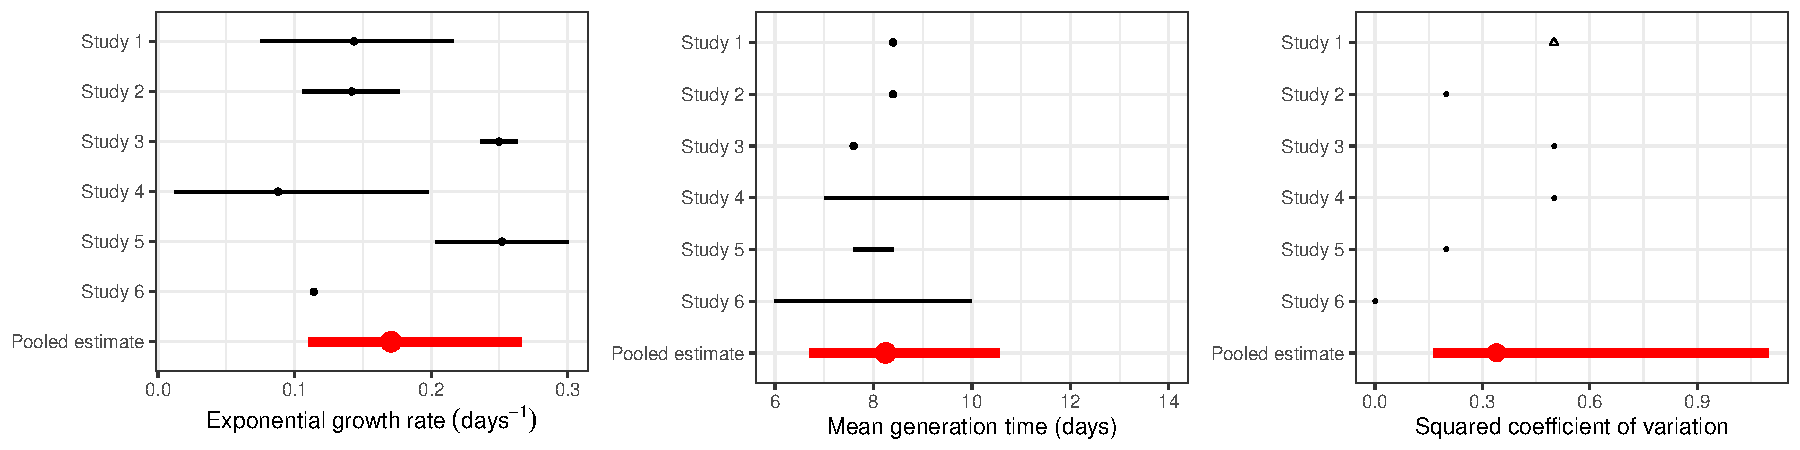
\includegraphics[width=\textwidth]{compare_assumption.pdf}
\caption{
\textbf{Comparisons of the reported parameter values with our pooled estimates.}
We inferred point estimates (black), uniform distributions (orange) or confidence\DIFaddbeginFL \DIFaddFL{/credible }\DIFaddendFL intervals (purple) for each parameter from each study, and combined them into pooled estimates \DIFaddbeginFL \DIFaddFL{using a Bayesian multilevel model }\DIFaddendFL (red\DIFdelbeginFL \DIFdelFL{; see text}\DIFdelendFL ).
\DIFaddbeginFL \DIFaddFL{Points represent medians calculated from the parameter set $(\bar{G}_{i}, \kappa_{i}, r_{i})$ for each study $i$ (orange and purple).
Error bars represent 95\% equi-tailed quantiles calculated from the parameter set $(\bar{G}_{i}, \kappa_{i}, r_{i})$ for each study $i$.
Red density plots represent distributions of 2000 posterior samples.
}\DIFaddendFL Open triangle: we assumed $\kappa=0.5$ for Study 2 which does not report generation-interval \DIFdelbeginFL \DIFdelFL{dispersion}\DIFdelendFL \DIFaddbeginFL \DIFaddFL{assumptions}\DIFaddendFL .
}
\label{fig:assumption}
\end{figure}

\fref{eff} shows how propagating uncertainty in \DIFdelbegin \DIFdel{different combinations would }\DIFdelend \DIFaddbegin \DIFadd{underlying parameters }\DIFaddend affect estimates and CIs for \Ro. 
For illustrative purposes, we use our pooled estimates, which may represent a reasonable proxy for the state of knowledge as of January 23--26\DIFaddbegin \DIFadd{, 2020 }\DIFaddend (\fref{eff}A).
Comparing the \DIFdelbegin \DIFdel{models }\DIFdelend \DIFaddbegin \DIFadd{estimates }\DIFaddend that include only some sources of uncertainty to the \DIFdelbegin \DIFdel{``all'' model}\DIFdelend \DIFaddbegin \DIFadd{pooled estimate ($\Rpool = 3.0$; 95\% CI: 2.1--4.6; see `all' in \fref{eff})}\DIFaddend , we see that propagating error from the growth rate (\DIFdelbegin \DIFdel{which }\DIFdelend \DIFaddbegin \DIFadd{as done by }\DIFaddend all but one \DIFdelbegin \DIFdel{of the studies revieweddid}\DIFdelend \DIFaddbegin \DIFadd{studies reviewed}\DIFaddend ) is absolutely crucial: \DIFdelbegin \DIFdel{the middle bar (``GI mean''}\DIFdelend \DIFaddbegin \DIFadd{uncertainty in the pooled estimates for both middle bars ($\mu_G$ and $\mu_\kappa$}\DIFaddend ), which \DIFdelbegin \DIFdel{lacks }\DIFdelend \DIFaddbegin \DIFadd{lack }\DIFaddend growth-rate uncertainty, \DIFdelbegin \DIFdel{is relatively }\DIFdelend \DIFaddbegin \DIFadd{are overly }\DIFaddend narrow.
In this case, propagating error from the mean generation interval has \DIFaddbegin \DIFadd{a }\DIFaddend negligible effect compared to propagating the uncertainty in $r$.
Uncertainty in the generation-interval dispersion \DIFaddbegin \DIFadd{$\kappa$ }\DIFaddend also has important effects \DIFdelbegin \DIFdel{as it determines the functional form of the relationship between $r$ and }%DIFDELCMD < \Ro %%%
\DIFdel{(compare ``growth rate + GI mean'' with ``all'').
For example, reducing the dispersion parameter $\kappa$ from 1 (assuming exponentially distributed generation intervals) to 0 (assuming fixed generation intervals)changes the $r$--}%DIFDELCMD < \Ro%%%
\DIFdel{\ relationship from linear to exponential , therefore increasing the sensitivity of }%DIFDELCMD < \Ro %%%
\DIFdel{estimates to $r$ and $\bar G$.
}\DIFdelend \DIFaddbegin \DIFadd{(compare $\mu_G$ credible intervals with $\mu_\kappa$ credible intervals in \fref{eff}A).
However, our estimate of }\Rpool \DIFadd{is relatively insensitive to our assumption of $\kappa=0.5$ for Study 2: assuming $\kappa=0.1$ gives $\Rpool = 3.0$ (95\% CI: 2.2--4.7), whereas assuming $\kappa=0.9$ gives $\Rpool = 2.9$ (95\% CI: 2.1--4.4).
}\DIFaddend 

\DIFaddbegin \DIFadd{We further explore how the effects of uncertainties in generation-interval distributions change when the exponential growth rate is more certain.
This hypothetical example reflects scenarios, in which increased data availability allows researchers to estimate $r$ with more certainty.
To simulate estimates of the exponential growth rate with stronger confidence, we use $\hat{\mu}_r = (\mu_r + 3\times\mathrm{median}(\mu_r))/4$ instead of $\mu_r$ (\fref{eff}B); 
then $\hat{\mu}_r$ has the same median as $\mu_r$ but the associated 95\% CI is 4 times narrower (0.16--0.19 $\textrm{days}^{-1}$).
}\DIFaddend As uncertainty associated with the exponential growth rate decreases, accounting for uncertainties in generation intervals becomes even more important\DIFdelbegin \DIFdel{(\fref{eff}B)}\DIFdelend .
Propagating error only from the growth rate \DIFaddbegin \DIFadd{($\hat{\mu}_r$ in \fref{eff}B) }\DIFaddend gives very narrow \DIFdelbegin \DIFdel{confidence }\DIFdelend \DIFaddbegin \DIFadd{credible }\DIFaddend intervals in this case. 
\DIFdelbegin \DIFdel{Likewise, propagating }\DIFdelend \DIFaddbegin \DIFadd{Propagating }\DIFaddend errors from the \DIFdelbegin \DIFdel{growth rate and the }\DIFdelend mean generation interval \DIFdelbegin \DIFdel{gives wider but still too narrow confidence intervals.
We expect this hypothetical example to better reflect more recent scenarios, as increased data availability will allow researchers to estimate $r$ with more certainty.
}\DIFdelend \DIFaddbegin \DIFadd{($\mu_G$ in \fref{eff}B) or generation-interval dispersion ($\mu_\kappa$ in \fref{eff}B) gives more realistic but still narrow credible intervals.
}\DIFaddend 

\begin{figure}[!ht]
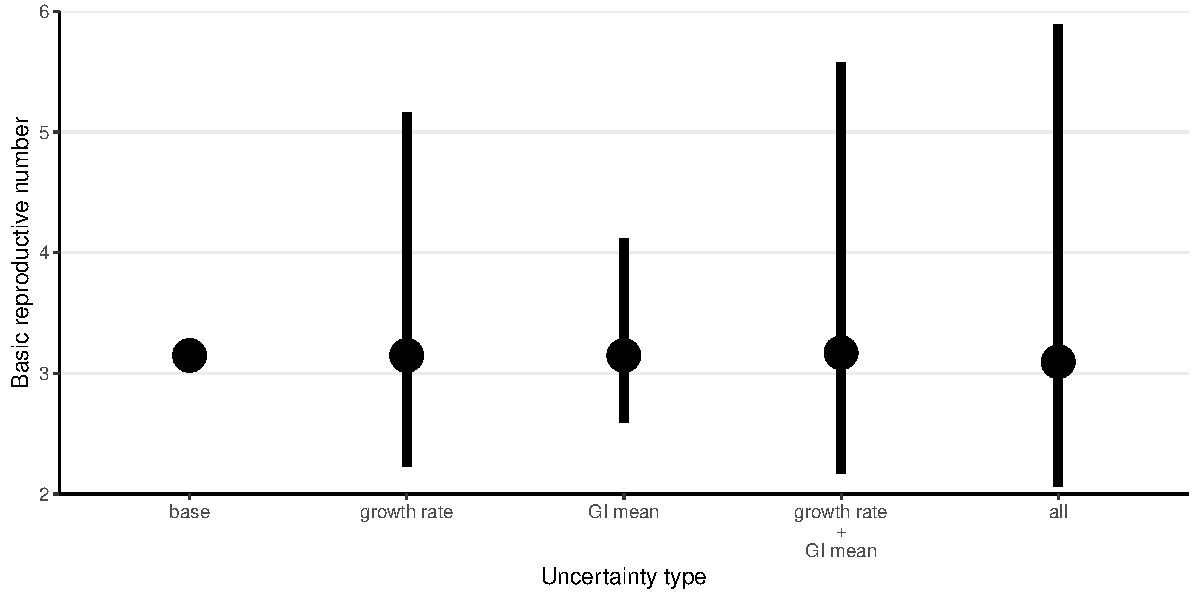
\includegraphics[width=\textwidth]{figure2.pdf}
\caption{
  \textbf{Effects of $r$, $\bar G$, and $\kappa$ on the estimates of \Ro.}
We compare estimates of \Ro under \DIFdelbeginFL \DIFdelFL{five }\DIFdelendFL \DIFaddbeginFL \DIFaddFL{nine }\DIFaddendFL scenarios that propagate different \DIFdelbeginFL \DIFdelFL{combinations of }\DIFdelendFL \DIFaddbeginFL \DIFaddFL{parameter }\DIFaddendFL uncertainties (A) based on our pooled estimates ($\mu_r$, $\mu_G$, and $\mu_\kappa$) and (B) assuming a 4-fold reduction in uncertainty of our pooled estimate of the exponential growth rate (using \DIFdelbeginFL \DIFdelFL{$(\mu_r + 3\times\mathrm{median}(\mu_r))/4$, }\DIFdelendFL \DIFaddbeginFL \DIFaddFL{$\hat{\mu}_r = (\mu_r + 3\times\mathrm{median}(\mu_r))/4$ }\DIFaddendFL instead \DIFaddbeginFL \DIFaddFL{of $\mu_r$}\DIFaddendFL ).
\DIFdelbeginFL \textbf{\DIFdelFL{base}}%DIFAUXCMD
\DIFdelFL{: }\DIFdelendFL \DIFaddbeginFL \DIFaddFL{Each uncertainty type represents }\DIFaddendFL \Ro estimates based \DIFdelbeginFL \DIFdelFL{on }\DIFdelendFL the \DIFdelbeginFL \DIFdelFL{median estimates }\DIFdelendFL \DIFaddbeginFL \DIFaddFL{posterior distributions }\DIFaddendFL of \DIFaddbeginFL \DIFaddFL{one of three parameters (}\DIFaddendFL $\mu_r$, $\mu_G$, and $\mu_\kappa$\DIFdelbeginFL \DIFdelFL{.
}\textbf{\DIFdelFL{growth rate}}%DIFAUXCMD
\DIFdelFL{: }%DIFDELCMD < \Ro %%%
\DIFdelFL{estimates based on the the posterior distribution of $\mu_r$ }\DIFdelendFL \DIFaddbeginFL \DIFaddFL{) }\DIFaddendFL while using median estimates of \DIFdelbeginFL \DIFdelFL{$\mu_G$ and $\mu_\kappa$}\DIFdelendFL \DIFaddbeginFL \DIFaddFL{two other parameters}\DIFaddendFL .
\DIFdelbeginFL \textbf{\DIFdelFL{GI mean}}%DIFAUXCMD
\DIFdelFL{: }\DIFdelendFL \DIFaddbeginFL \DIFaddFL{The `none' type represents }\DIFaddendFL \Ro \DIFdelbeginFL \DIFdelFL{estimates }\DIFdelendFL \DIFaddbeginFL \DIFaddFL{estimate }\DIFaddendFL based on the \DIFdelbeginFL \DIFdelFL{the posterior distribution of $\mu_G$ while using }\DIFdelendFL median estimates of $\mu_r$\DIFaddbeginFL \DIFaddFL{, $\mu_G$, }\DIFaddendFL and $\mu_\kappa$.
\DIFdelbeginFL \textbf{\DIFdelFL{growth rate + GI mean}}%DIFAUXCMD
\DIFdelFL{: }\DIFdelendFL \DIFaddbeginFL \DIFaddFL{The `all' type represents }\DIFaddendFL \Ro estimates based on the \DIFdelbeginFL \DIFdelFL{the }\DIFdelendFL joint posterior distributions of  $\mu_r$\DIFdelbeginFL \DIFdelFL{and $\mu_G$ while using a median estimate of $\mu_\kappa$.
}\textbf{\DIFdelFL{all}}%DIFAUXCMD
\DIFdelFL{: }%DIFDELCMD < \Ro %%%
\DIFdelFL{estimates based on the joint posterior distributions of  $\mu_r$}\DIFdelendFL , $\mu_G$, and $\mu_\kappa$ \DIFaddbeginFL \DIFaddFL{(also corresponds to }\Rpool\DIFaddFL{)}\DIFaddendFL .
\DIFaddbeginFL \DIFaddFL{Points represent the median estimates.
}\DIFaddendFL Vertical \DIFdelbeginFL \DIFdelFL{lines }\DIFdelendFL \DIFaddbeginFL \DIFaddFL{error bars }\DIFaddendFL represent the 95\% \DIFdelbeginFL \DIFdelFL{confidence }\DIFdelendFL \DIFaddbeginFL \DIFaddFL{credible }\DIFaddendFL intervals.
}
\label{fig:eff}
\end{figure}

\DIFdelbegin \DIFdel{We also compare the estimates of }%DIFDELCMD < \Ro %%%
\DIFdel{across different studies by 
replacing their values of $r$, $\bar G$, and $\kappa$ with our pooled estimates ($\mu_r$, $\mu_G$, and $\mu_\kappa$, respectively) one at a time and recalculating the basic reproductive number }%DIFDELCMD < \Ro %%%
\DIFdel{(\fref{R0}).
This procedure allows us to assess the sensitivity of the estimates of }%DIFDELCMD < \Ro %%%
\DIFdel{across appropriate ranges of uncertainties.
We find that incorporating uncertainties one at a time increases the width of the confidence intervals in all but 7 cases .
We estimate narrower confidence intervals for Study }\DIFdelend \DIFaddbegin \DIFadd{Finally, \fref{R0} compares the base estimates (based on $r_i$, $\bar G_i$, and $\kappa_i$ for each study $i$) and 21 substitute estimates (}\DIFaddend 3 \DIFdelbegin \DIFdel{, Study 6, and Study }\DIFdelend \DIFaddbegin \DIFadd{parameter substitutions $\times$ }\DIFaddend 7 \DIFdelbegin \DIFdel{when we account for proper uncertainties in the generation-interval dispersion because they assume a narrow generation-interval distribution (compare ``base'' with ``GI variation'');
when higher values of $\kappa$ are used, their estimates of }%DIFDELCMD < \Ro %%%
\DIFdel{become less sensitive to the values of $r$ and }\DIFdelend \DIFaddbegin \DIFadd{studies).
All but 8 substitute estimates have wider credible intervals compared to their corresponding base estimates --- the cases with more certain substitute estimates are the }\DIFaddend $\bar G$\DIFdelbegin \DIFdel{, giving narrower confidence intervals.
We estimate narrower confidence intervals for Study 5 and Study }\DIFdelend \DIFaddbegin \DIFadd{-substitute estimates for Study 1 and }\DIFaddend 7\DIFdelbegin \DIFdel{when we account for proper uncertainties in the mean generation interval (compare ``base'' with ``GI mean'') because the range of uncertainty in the mean generation interval $\bar G$ they consider is much wider than the pooled range (\fref{assumption}).
Substituting the reported }\DIFdelend \DIFaddbegin \DIFadd{, }\DIFaddend $r$\DIFdelbegin \DIFdel{or $\bar G$ from }\DIFdelend \DIFaddbegin \DIFadd{-substitute estimates for }\DIFaddend Study 1 \DIFdelbegin \DIFdel{with our pooled estimates give narrower confidence intervals for similar reasons.
}%DIFDELCMD < 

%DIFDELCMD < %%%
\DIFdel{We find that accounting }\DIFdelend \DIFaddbegin \DIFadd{and 2, and  $\kappa$-substitute estimates }\DIFaddend for \DIFaddbegin \DIFadd{Study 3, 6, and 7.
Accounting for }\DIFaddend uncertainties in the estimate of $r$ has the largest effect on the estimates of \Ro\ in most cases (\fref{R0}).
For example, \DIFdelbegin \DIFdel{recalculating }\DIFdelend \DIFaddbegin \DIFadd{the $r$-substitute estimate of }\DIFaddend \Ro for Study 7 \DIFdelbegin \DIFdel{by using our pooled estimate of $r$ gives }\DIFdelend \DIFaddbegin \DIFadd{is }\DIFaddend $\Ro = 3.9$ (95\% CI: 2.3--8\DIFdelbegin \DIFdel{.6}\DIFdelend \DIFaddbegin \DIFadd{.8}\DIFaddend ), which is much wider than the uncertainty range \DIFdelbegin \DIFdel{they reported }\DIFdelend \DIFaddbegin \DIFadd{reported by the authors }\DIFaddend (2.0--3.1).
\DIFdelbegin \DIFdel{There are two explanations for this result.
First, even though }\DIFdelend \DIFaddbegin \DIFadd{This is consistent with our earlier results (\fref{eff}) that demonstrated the importance of accounting for uncertainty in }\DIFaddend the exponential growth rate $r$\DIFdelbegin \DIFdel{and the mean generation interval $\bar G$ have identical mathematical effects on }%DIFDELCMD < \Ro %%%
\DIFdel{in our framework (\eref{gamma} in Methods) }\DIFdelend \DIFaddbegin \DIFadd{.
We also note that the pooled estimate of the basic reproductive number ($\Rpool = 3.0$; 95\% CI: 2.1--4.6) has wider credible intervals than the base estimates in all cases except for Study 6.
}

\begin{figure}[!th]
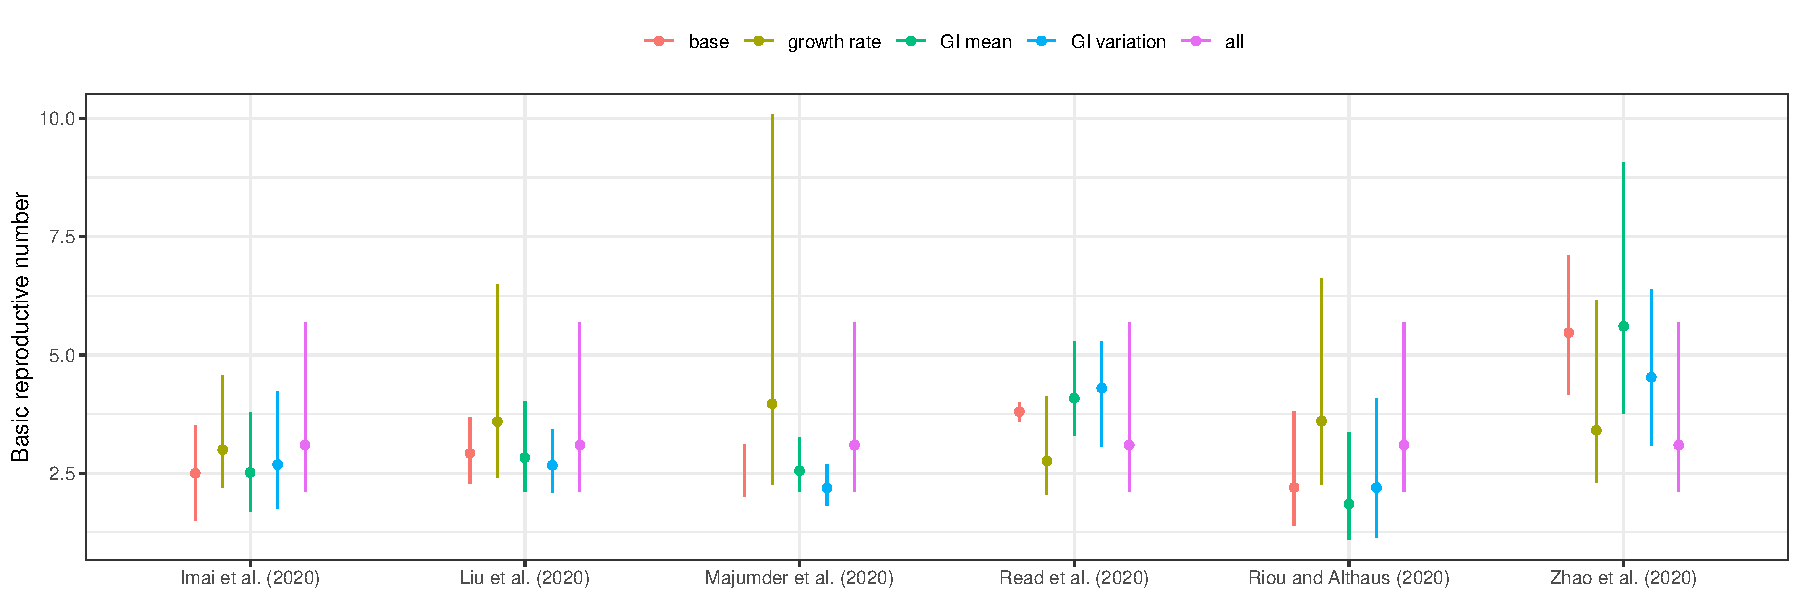
\includegraphics[width=\textwidth]{compare_R0.pdf}
\caption{
\textbf{\DIFaddFL{Sensitivity of the reported }\Ro \DIFaddFL{estimates with respect to our pooled estimates of the underlying parameters.}}
\DIFaddFL{We calculate substitute estimates by replacing the reported parameter values (growth rate $r$, mean generation interval $\bar G$, and generation-interval dispersion $\kappa$) with our corresponding pooled estimates ($\mu_r$, $\mu_G$, and $\mu_\kappa$) one at a time and recalculate }\Ro\DIFaddFL{.
The pooled estimate represents }\Rpool\DIFaddFL{, which is calculated from the joint posterior distribution of $\mu_r$, $\mu_G$, and $\mu_\kappa$;
this corresponds to replacing all reported parameter values with our pooled estimates, which gives identical results across all studies.
Points represent the medians of our base, substitute, and pooled estimates.
Vertical error bars represent the 95\% credible intervals of our base, substitute, and pooled estimates.
Horizontal dashed lines represent the 95\% credible intervals of our pooled estimate.
}}
\label{fig:R0}
\end{figure}

\section{\DIFadd{Discussion}}

\DIFadd{Estimating the basic reproductive number }\Ro \DIFadd{is crucial for predicting the course of an outbreak and planning intervention strategies.
However, comparing disparate estimates of }\Ro \DIFadd{can be difficult when they rely on different methods and assumptions.
Here, we use a gamma approximation framework \mbox{%DIFAUXCMD
\citep{park2019practical} }\hspace{0pt}%DIFAUXCMD
to decompose }\Ro \DIFadd{estimates into three key quantities ($r$}\DIFaddend , \DIFaddbegin \DIFadd{$\bar G$, and $\kappa$) and apply a multilevel Bayesian framework to compare estimates of }\Ro \DIFadd{for the SARS-CoV-2 outbreak.
Our results demonstrate the importance of accounting for uncertainties associated with the underlying generation-interval distributions, including uncertainties in the degree of dispersion in the generation intervals.
}

\DIFadd{Our analysis shows that many early estimates of }\Ro \DIFadd{rely on overly confident assumptions.
The neglect of uncertainties in the generation-interval dispersion is particularly important because it determines the shape of the }\DIFaddend $r$\DIFdelbegin \DIFdel{is more influential in this case because it is associated with more uncertainty }\DIFdelend \DIFaddbegin \DIFadd{--}\Ro \DIFadd{relationship }\DIFaddend (\fref{assumption})\DIFdelbegin \DIFdel{.
Second, assuming }\DIFdelend \DIFaddbegin \DIFadd{:
reducing $\kappa$ from 1 (assuming exponentially distributed generation intervals) to 0 (assuming fixed generation intervals) changes the $r$--}\Ro \DIFadd{relationship from linear to exponential (see \eref{gamma}).
Assuming fixed parameter values here will lead to overly confident conclusions \mbox{%DIFAUXCMD
\citep{elderd2006uncertainty}}\hspace{0pt}%DIFAUXCMD
.
}

\DIFadd{The lack of uncertainty in the generation-interval dispersion further explains the sensitivity of }\Ro \DIFadd{estimates to the exponential growth rate, particularly in Study 7 (\fref{R0}).
Since Study 7 assumes }\DIFaddend a fixed generation interval ($\kappa=0$)\DIFdelbegin \DIFdel{makes the estimate of }\DIFdelend \DIFaddbegin \DIFadd{, they implicitly assume an exponential $r$--}\DIFaddend \Ro \DIFaddbegin \DIFadd{relationship, making their estimate }\DIFaddend too sensitive to $r$\DIFaddbegin \DIFadd{.
Similarly, the credible intervals associated with the base estimates of Studies 3 ($\kappa=0.2$), 6  ($\kappa=0.2$), and 7 ($\kappa=0$) are wider than the credible intervals associated with their corresponding $\kappa$-substitute estimates, which rely on wider generation-interval distributions ($\mu_\kappa=0.50$; 95\% CI: 0.26--1.10) and, therefore, are less sensitive to uncertainties in $r$ }\DIFaddend and $\bar G$.
One exception is Study 1: \DIFdelbegin \DIFdel{we find }\DIFdelend this estimate of \Ro is most sensitive to generation-interval dispersion $\kappa$\DIFdelbegin \DIFdel{.
This is because Study 1 }\DIFdelend \DIFaddbegin \DIFadd{,
because the study }\DIFaddend assumes an exponentially distributed generation interval ($\kappa=1$)\DIFdelbegin \DIFdel{: estimates }\DIFdelend \DIFaddbegin \DIFadd{. 
Estimates }\DIFaddend that rely on this assumption \DIFdelbegin \DIFdel{make }\DIFdelend \DIFaddbegin \DIFadd{implicitly assume a linear $r$--}\DIFaddend \Ro \DIFdelbegin \DIFdel{relatively insensitive and thus tend to have particularly narrow confidence intervals}\DIFdelend \DIFaddbegin \DIFadd{relationship}\DIFaddend .

\DIFdelbegin %DIFDELCMD < \begin{figure}[!th]
%DIFDELCMD < 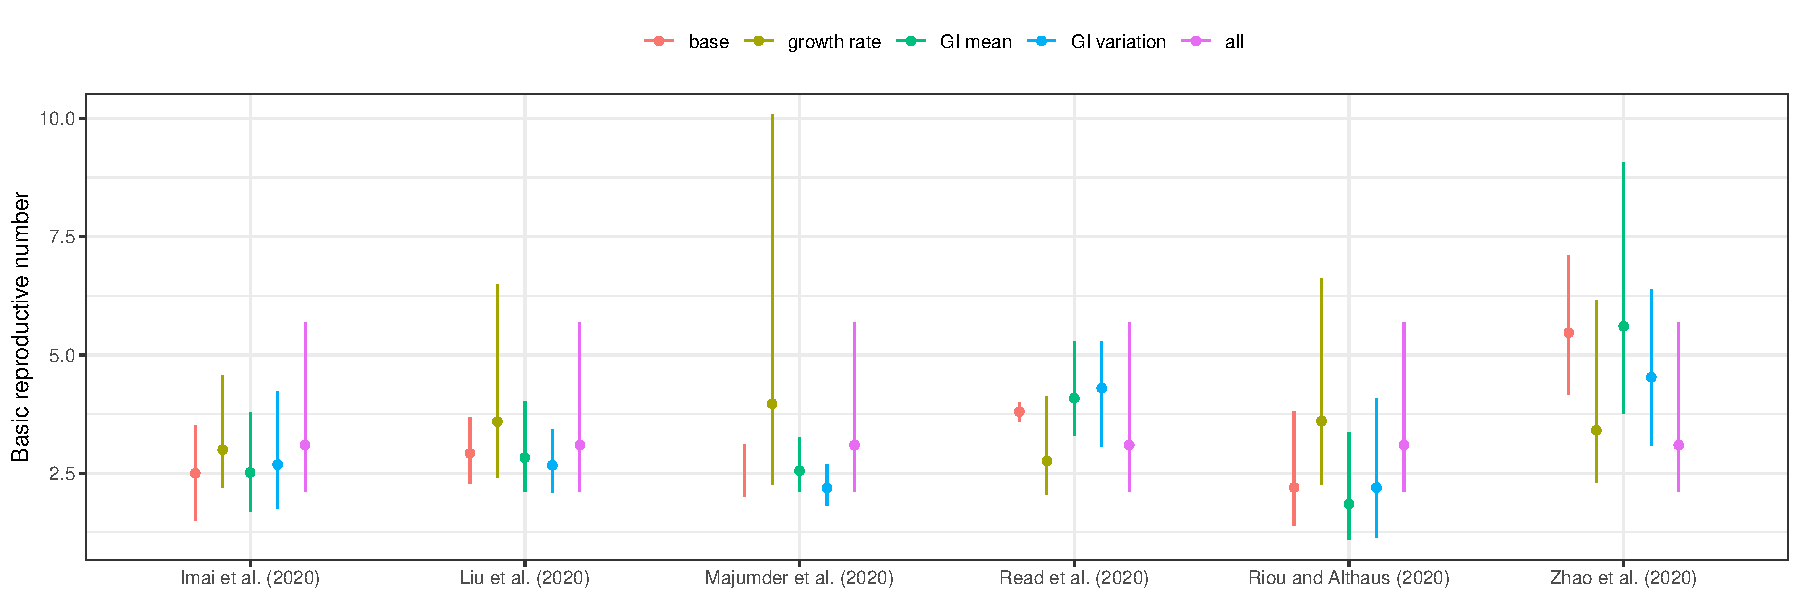
\includegraphics[width=\textwidth]{compare_R0.pdf}
%DIFDELCMD < %%%
%DIFDELCMD < \caption{%
{%DIFAUXCMD
\textbf{\DIFdelFL{Sensitivity of the reported }%DIFDELCMD < \Ro %%%
\DIFdelFL{estimates with respect to our pooled estimates of the underlying parameters.}}
%DIFAUXCMD
\DIFdelFL{We replace the reported parameter values (growth rate $r$, GI mean $\bar G$, and GI variation $\kappa$) with our corresponding pooled estimates ($\mu_r$, $\mu_G$, and $\mu_\kappa$) one at a time and recalculate }%DIFDELCMD < \Ro %%%
\DIFdelFL{(}\textbf{\DIFdelFL{growth rate}}%DIFAUXCMD
\DIFdelFL{, }\textbf{\DIFdelFL{GI mean}}%DIFAUXCMD
\DIFdelFL{, and }\textbf{\DIFdelFL{GI variation}}%DIFAUXCMD
\DIFdelFL{).
The pooled estimate of }%DIFDELCMD < \Ro %%%
\DIFdelFL{is calculated from the joint posterior distribution of $\mu_r$, $\mu_G$, and $\mu_\kappa$ (}\textbf{\DIFdelFL{all}}%DIFAUXCMD
\DIFdelFL{);
this corresponds to replacing all reported parameter values with our pooled estimates, which gives identical results across all studies.
Horizontal dashed lines represent the 95\% confidence intervals of our pooled estimate of }%DIFDELCMD < \Ro%%%
\DIFdelFL{.
The reported }%DIFDELCMD < \Ro %%%
\DIFdelFL{estimates (}\textbf{\DIFdelFL{base}}%DIFAUXCMD
\DIFdelFL{) have been adjusted to show the approximate 95\% confidence interval using the probability distributions that we defined if they had relied on different measures for parameter uncertainties.
}}
%DIFAUXCMD
%DIFDELCMD < \label{fig:R0}
%DIFDELCMD < \end{figure}
%DIFDELCMD < 

%DIFDELCMD < %%%
\DIFdel{Finally, we incorporate all uncertainties by using posterior samples for $\mu_r$, $\mu_G$, and $\mu_\kappa$ to recalculate }\DIFdelend \DIFaddbegin \DIFadd{As most studies rely on overly confident assumptions, the credible intervals associated with the base estimates of }\DIFaddend \Ro \DIFdelbegin \DIFdel{and compare it with the reported }%DIFDELCMD < \Ro %%%
\DIFdel{estimates .
Our estimated }%DIFDELCMD < \Ro %%%
\DIFdel{from the pooled distribution has a median of 2.9 (}\DIFdelend \DIFaddbegin \DIFadd{should tend to be narrower than the credible intervals of the pooled estimate ($\Rpool = 3.0$; }\DIFaddend 95\% CI: 2.1--4\DIFdelbegin \DIFdel{.5}\DIFdelend \DIFaddbegin \DIFadd{.6}\DIFaddend ).
While the point estimate of \DIFdelbegin %DIFDELCMD < \Ro %%%
\DIFdelend \DIFaddbegin \Rpool \DIFaddend is similar to other reported values from this date range, \DIFdelbegin \DIFdel{the confidence intervals are wider than }\DIFdelend \DIFaddbegin \DIFadd{its credible interval is wider than the credible intervals of the base estimates of }\DIFaddend all but one study.
This result does not \DIFdelbegin \DIFdel{imply that assumptions based on }\DIFdelend \DIFaddbegin \DIFadd{mean that assumptions underlying }\DIFaddend the pooled estimate are too weak;
\DIFdelbegin \DIFdel{we believe that this confidence }\DIFdelend \DIFaddbegin \DIFadd{rather, this credible }\DIFaddend interval more accurately reflects the level of uncertainties present in the information that was available when these models were fitted.
In fact, because the pooled estimate does not account for overlap in data sources used by the models, \DIFdelbegin \DIFdel{we feel that }\DIFdelend it is more likely to be over-confident than under-confident.
\DIFdelbegin \DIFdel{Our }\DIFdelend \DIFaddbegin \DIFadd{Because our }\DIFaddend median estimate averages over the various studies, \DIFdelbegin \DIFdel{and therefore }\DIFdelend particular studies have higher or lower median estimates.
\DIFdelbegin \DIFdel{We note in particularthat}\DIFdelend \DIFaddbegin \DIFadd{In particular}\DIFaddend , while the baseline example we used from Study 6 may appear to be an outlier, the authors of this study also explore different scenarios involving changes in reporting rate over time, under which their estimates of \Ro are similar to other reported estimates.
\DIFdelbegin \DIFdel{Here, our focus is on estimating uncertainty, not on identifying potential explanations for these discrepancies.
}\DIFdelend 

\DIFdelbegin \section{\DIFdel{Discussion}}
%DIFAUXCMD
\addtocounter{section}{-1}%DIFAUXCMD
%DIFDELCMD < 

%DIFDELCMD < %%%
\DIFdel{Estimating the basic reproductive number }%DIFDELCMD < \Ro %%%
\DIFdel{is crucial for predicting the course of an outbreak and planning intervention strategies.
Here, we use a gamma approximation \mbox{%DIFAUXCMD
\citep{park2019practical} }\hspace{0pt}%DIFAUXCMD
to decompose }%DIFDELCMD < \Ro %%%
\DIFdel{estimates into three key quantities ($r$, $\bar G$, and $\kappa$) and apply a multilevel Bayesian framework to compare estimates of }%DIFDELCMD < \Ro %%%
\DIFdel{for the novel coronavirus outbreak.
Our results demonstrate the importance of accounting for uncertainties associated with the underlying generation-interval distributions, including uncertainties in the amount of dispersion in the generation intervals.
Our analysis of individual studies shows that many early estimates of }%DIFDELCMD < \Ro %%%
\DIFdel{rely on strong assumptions.
}%DIFDELCMD < 

%DIFDELCMD < %%%
\DIFdelend Of the seven studies that we \DIFdelbegin \DIFdel{reviewed, two }\DIFdelend \DIFaddbegin \DIFadd{review, at least one }\DIFaddend of them directly fit their models to \DIFaddbegin \DIFadd{the }\DIFaddend cumulative number of confirmed cases.
This approach \DIFdelbegin \DIFdel{can be }\DIFdelend \DIFaddbegin \DIFadd{is }\DIFaddend appealing because of its simplicity and apparent robustness, but fitting a model to cumulative incidence \DIFdelbegin \DIFdel{instead of raw incidence can both bias parameters and give overly narrow confidence intervals , if the resulting non-independent error structures are not taken into account \mbox{%DIFAUXCMD
\citep{ma2014estimating, king2015avoidable}}\hspace{0pt}%DIFAUXCMD
.
Naive fits to cumulative incidence data should therefore be avoided.
}\DIFdelend \DIFaddbegin \DIFadd{neglects autocorrelation between successive counts of cumulative cases. 
As a result, this approach both biases parameter estimates and gives overly narrow credible intervals \mbox{%DIFAUXCMD
\citep{ma2014estimating, king2015avoidable}}\hspace{0pt}%DIFAUXCMD
.
Narrow uncertainties in the estimates of the exponential growth rate are probably driven by this approach.
}\DIFaddend 

Many sources of noise affect real-world incidence data, including both dynamical, or ``process'', noise (randomness that directly or indirectly affects \DIFdelbegin \DIFdel{disease transmission}\DIFdelend \DIFaddbegin \DIFadd{the actual number of cases occurring}\DIFaddend ); and observation noise (randomness underlying how many of \DIFdelbegin \DIFdel{the true }\DIFdelend \DIFaddbegin \DIFadd{these }\DIFaddend cases are reported).  
Disease modelers face the choice of incorporating one or both of these in their data-fitting and modeling steps. 
\DIFdelbegin \DIFdel{This }\DIFdelend \DIFaddbegin \DIFadd{Neglecting one or the other }\DIFaddend is not always a serious problem, particularly if the goal is inferring parameters rather than directly making forecasts \citep{ma2014estimating}.
Modelers should\DIFdelbegin \DIFdel{however be aware of the possibility that ignoring one kind of error }\DIFdelend \DIFaddbegin \DIFadd{, however, be aware that oversimplifying the error model }\DIFaddend can give overly narrow \DIFdelbegin \DIFdel{confidence }\DIFdelend \DIFaddbegin \DIFadd{credible }\DIFaddend intervals \citep{king2015avoidable,taylor2016stochasticity}.

\DIFdelbegin \DIFdel{There are }\DIFdelend \DIFaddbegin \DIFadd{Our simple framework neglects some }\DIFaddend other important phenomena\DIFdelbegin \DIFdel{not covered by our simple framework}\DIFdelend .
Examples that seem relevant to this outbreak include: changing reporting rates\DIFdelbegin \DIFdel{, }\DIFdelend \DIFaddbegin \DIFadd{; }\DIFaddend reporting delays (including the effects of weekends and holidays)\DIFdelbegin \DIFdel{, }\DIFdelend \DIFaddbegin \DIFadd{; }\DIFaddend and changing generation intervals.
For emerging pathogens such as SARS-CoV-2, there may be an early period of time when the reporting rate is very low due to limited awareness or diagnostic resources;
for example, \cite{zhaoncov} (Study 6) demonstrated that estimates of \Ro can change from 5.47 (95\% CI: 4.16--7.10) to 3.30 (95\% CI: 2.73--3.96) when they assume 2-fold changes in the reporting rate between January 17, when the official diagnostic guidelines were released \citep{who17protocol}, and January 20.
Delays between key epidemiological timings (e.g., infection, symptom onset, and detection) can also shift the shape of an observed epidemic curve and, therefore, affect parameter estimates as well as predictions of the course of an outbreak \citep{tariq2019assessing}.
Even though a constant delay between infection and detection may not affect the estimate of the growth rate, it can still affect the associated \DIFdelbegin \DIFdel{confidence intervals.
}\DIFdelend \DIFaddbegin \DIFadd{credible intervals.
Other factors related to reporting --- including changes in case definition, saturation in diagnostic test capacity, transparency of data, and representativeness of samples --- will also affect estimation and inference.
}\DIFaddend Finally, generation intervals can become shorter throughout an epidemic as intervention strategies \DIFdelbegin \DIFdel{, such as quarantine, }\DIFdelend \DIFaddbegin \DIFadd{such as isolation of detected cases }\DIFaddend can reduce the infectious period \citep{hethcote2002effects}\DIFaddbegin \DIFadd{;
since we are primarily focusing on the outbreak in Wuhan City before confinement, generation intervals are unlikely to vary significantly.
All of these factors, including fitting to cumulative curves or ignoring process errors, affect the estimation of the exponential growth rate (as well as the associated uncertainties), which in turn affects the estimation of the basic reproductive number}\DIFaddend .
\DIFdelbegin \DIFdel{Accounting for these factorsis crucial for making accurate inferences.
}\DIFdelend 

Here, we \DIFdelbegin \DIFdel{focused }\DIFdelend \DIFaddbegin \DIFadd{focus }\DIFaddend on the estimates of \Ro that \DIFdelbegin \DIFdel{were }\DIFdelend \DIFaddbegin \DIFadd{are }\DIFaddend published within a very short time frame (January 23--26\DIFdelbegin \DIFdel{).
}\DIFdelend \DIFaddbegin \DIFadd{, 2020).
Since these estimates were published as pre-prints, rather than in peer-reviewed journals, the quality of the analyses as well as the resulting estimates were not necessarily finalized.
For example, Study 4 initially estimated $\Ro = 3.8$ (95\% CI: 3.6--4.0; \mbox{%DIFAUXCMD
\cite{readncov}}\hspace{0pt}%DIFAUXCMD
) but revised their estimate on January 28, 2020 to $\Ro = 3.11$ (95\% CI: 2.39--4.13; \mbox{%DIFAUXCMD
\cite{readncov2}}\hspace{0pt}%DIFAUXCMD
);
we do not include their revised estimates in our analysis in order to focus on available information at the very beginning of the outbreak.
Some studies also lack detailed description of their methods, data, and/or assumptions.
The variation in quality of these analyses adds further uncertainty to their results that is not captured by their uncertainty quantification (e.g., reported credible intervals) or by our analysis.
}

\DIFaddend During early phases of an outbreak, it is reasonable to assume that the epidemic grows exponentially \citep{anderson1991infectious}.
However, as the number of susceptible individuals decreases \DIFdelbegin \DIFdel{, the epidemicwill saturate, and }\DIFdelend \DIFaddbegin \DIFadd{or behavior changes in response to perception of the epidemic, the growth rate will decrease: }\DIFaddend estimates of $r$ used for \Ro should account for the possibility that $r$ is decreasing through time.
Although our analysis \DIFdelbegin \DIFdel{only reflects a snapshot of a fast-moving }\DIFdelend \DIFaddbegin \DIFadd{applies strictly to the earliest stages of an }\DIFaddend epidemic, we expect certain lessons to hold \DIFdelbegin \DIFdel{: confidence }\DIFdelend \DIFaddbegin \DIFadd{more generally: credible }\DIFaddend intervals must combine \DIFdelbegin \DIFdel{different }\DIFdelend \DIFaddbegin \DIFadd{as many }\DIFaddend sources of uncertainty \DIFaddbegin \DIFadd{as possible}\DIFaddend . 
In fact, as epidemics progress and more data becomes available, it is likely that inferences about exponential growth rate (and other epidemiological parameters) will \DIFaddbegin \DIFadd{generally }\DIFaddend become more precise; thus the risk of over-confidence \DIFaddbegin \DIFadd{(}\DIFaddend when uncertainty about the generation-interval distribution is neglected\DIFaddbegin \DIFadd{) }\DIFaddend will become greater.
\DIFaddbegin \DIFadd{Incorporating estimates of the dynamics of susceptibility (e.g., using properly calibrated serological studies \mbox{%DIFAUXCMD
\citep{metcalf2016use}}\hspace{0pt}%DIFAUXCMD
) is also important for characterizing transmission as the outbreak progresses.
}\DIFaddend 

We strongly emphasize the value of attention to accurate characterization of the transmission chains via \DIFaddbegin \DIFadd{both }\DIFaddend contact tracing and \DIFdelbegin \DIFdel{better }\DIFdelend \DIFaddbegin \DIFadd{improved }\DIFaddend statistical frameworks for inferring generation-interval distributions from such data \citep{britton2019estimation}.
A combined effort between public-health workers and modelers in this direction \DIFdelbegin \DIFdel{will be crucial }\DIFdelend \DIFaddbegin \DIFadd{is crucial both }\DIFaddend for predicting the course of an epidemic and \DIFaddbegin \DIFadd{for }\DIFaddend controlling it.
We also emphasize the value of transparency from modelers.
Model estimates during an outbreak, even in pre-prints, should include code links and complete explanations.
\DIFdelbegin \DIFdel{We suggest using methods }\DIFdelend \DIFaddbegin \DIFadd{Methods }\DIFaddend based on open-source tools allow for maximal reproducibility \DIFaddbegin \DIFadd{\mbox{%DIFAUXCMD
\citep{barton2020call}}\hspace{0pt}%DIFAUXCMD
}\DIFaddend .

\DIFdelbegin \DIFdel{In summary, we }\DIFdelend \DIFaddbegin \DIFadd{Despite our focus on estimating }\Ro \DIFadd{at the onset of an outbreak, many of the issues persist now. 
For example, \mbox{%DIFAUXCMD
\cite{flaxman2020estimating} }\hspace{0pt}%DIFAUXCMD
recently estimated the basic reproductive number for SARS-CoV-2 outbreaks in 11 European countries to be around 3.87 (3.01--4.66), on average.
While these estimates appear to be broadly consistent with earlier estimates from China, comparing the exponential growth rate and the underlying generation-interval distributions suggest otherwise.
The later paper assumes a shorter mean generation interval ($\bar G = 6.5\,\textrm{days}$) but similar generation-interval dispersion ($\kappa = 0.38$);
based on these values, the exponential growth rate has to be considerably higher ($r = 0.27\,\textrm{days}^{-1}$) to obtain $\Ro = 3.87$ than the exponential growth rate observed in China ($\mu_r = 0.17\,\textrm{days}^{-1}$; 95\% CI: 0.12--0.25 $\textrm{days}^{-1}$).
Naively comparing estimates of the basic reproductive number without accounting for differences in underlying assumptions can lead to over-interpretation of apparent differences in the estimates.
}

\DIFadd{We }\DIFaddend have provided a basis for comparing exponential-growth based estimates of \Ro and its associated uncertainty in terms of three components: the exponential growth rate, mean generation interval, and generation interval dispersion. 
We hope this framework will help researchers understand and reconcile disparate estimates of disease transmission early in an epidemic.

\pagebreak

\section*{Funding}

BMB and DJDE were supported by Natural Sciences and Engineering Research Council (NSERC). ML was supported by Canadian Institutes of Health Research (CIHR). The funders had no role in study design, data collection and analysis, decision to publish, or preparation of the manuscript.

\section*{Competing interests}

We declare no competing interests.

\section*{Acknowledgements}

We thank Daihai He for providing helpful comments on the manuscript.

\section*{Contribution}

SWP and JD developed the statistical framework\DIFaddbegin \DIFadd{, with contributions from all authors}\DIFaddend . 
SWP reviewed the published literature.
SWP performed the analysis.
SWP, BMB, and JD created the figures. 
SWP and JD wrote the first draft.
All authors contributed to the writing and approval of the final report.

\section*{Data availability}

\texttt{R} code is available in GitHub (\url{https://github.com/parksw3/nCoV_framework}).

\pagebreak

\bibliography{ncov_abbr}

\pagebreak
\appendix
\renewcommand\thefigure{A\arabic{figure}}
\setcounter{figure}{0}    
\section*{Appendix}

\begin{figure}[!h]
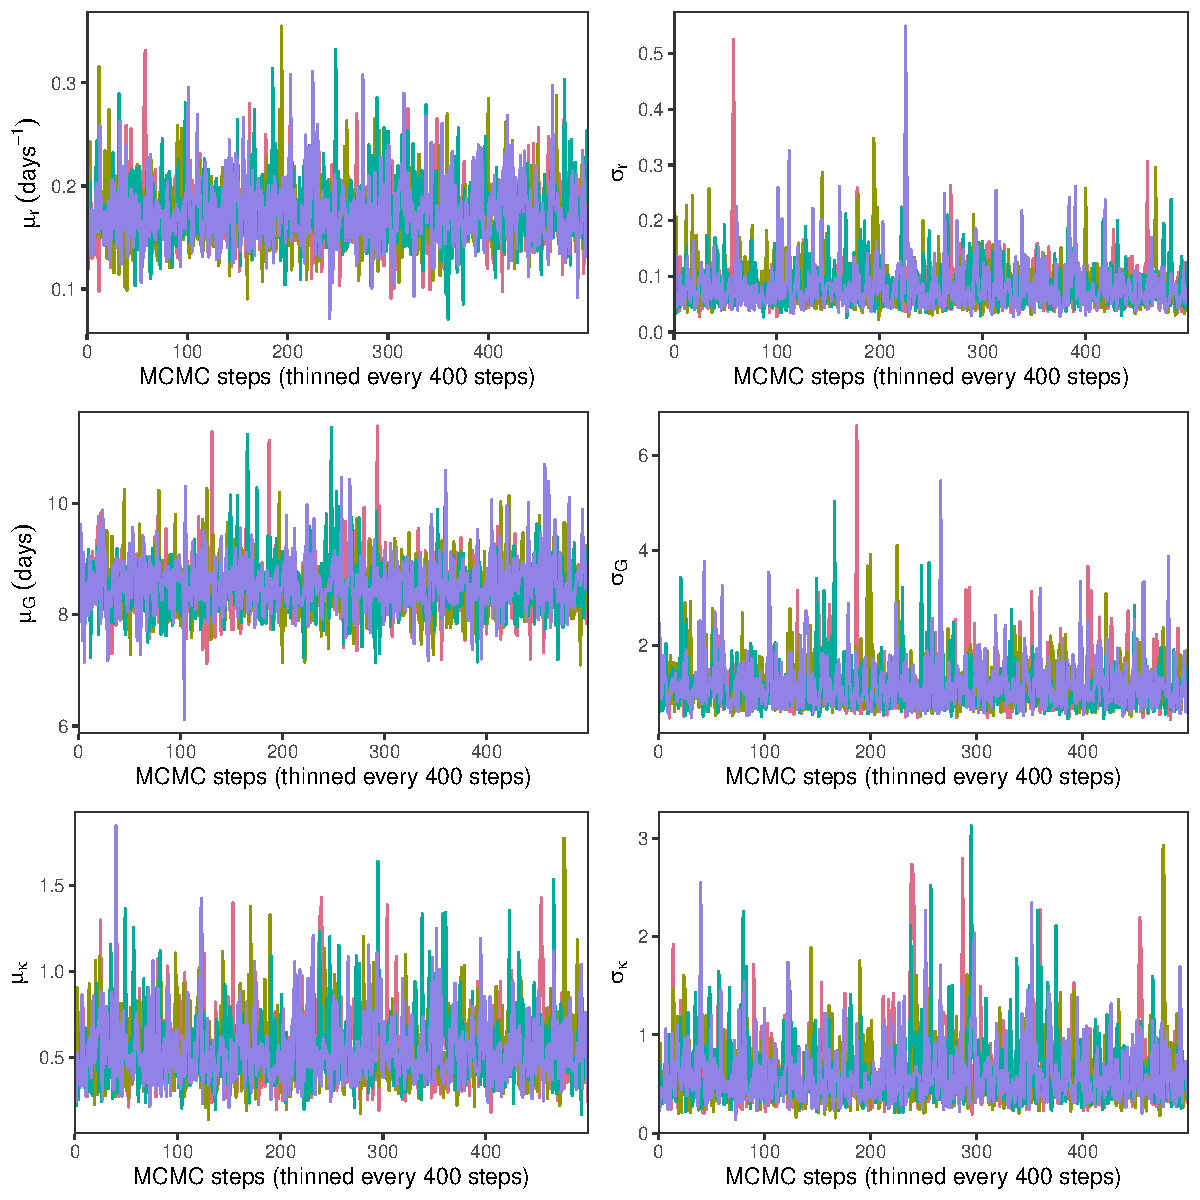
\includegraphics[width=\textwidth]{posterior_chain.pdf}
\caption{
\textbf{Trace plots of the multilevel model.}
Each chain is represented by a different color.
}
\end{figure}

\pagebreak

\begin{figure}[!h]
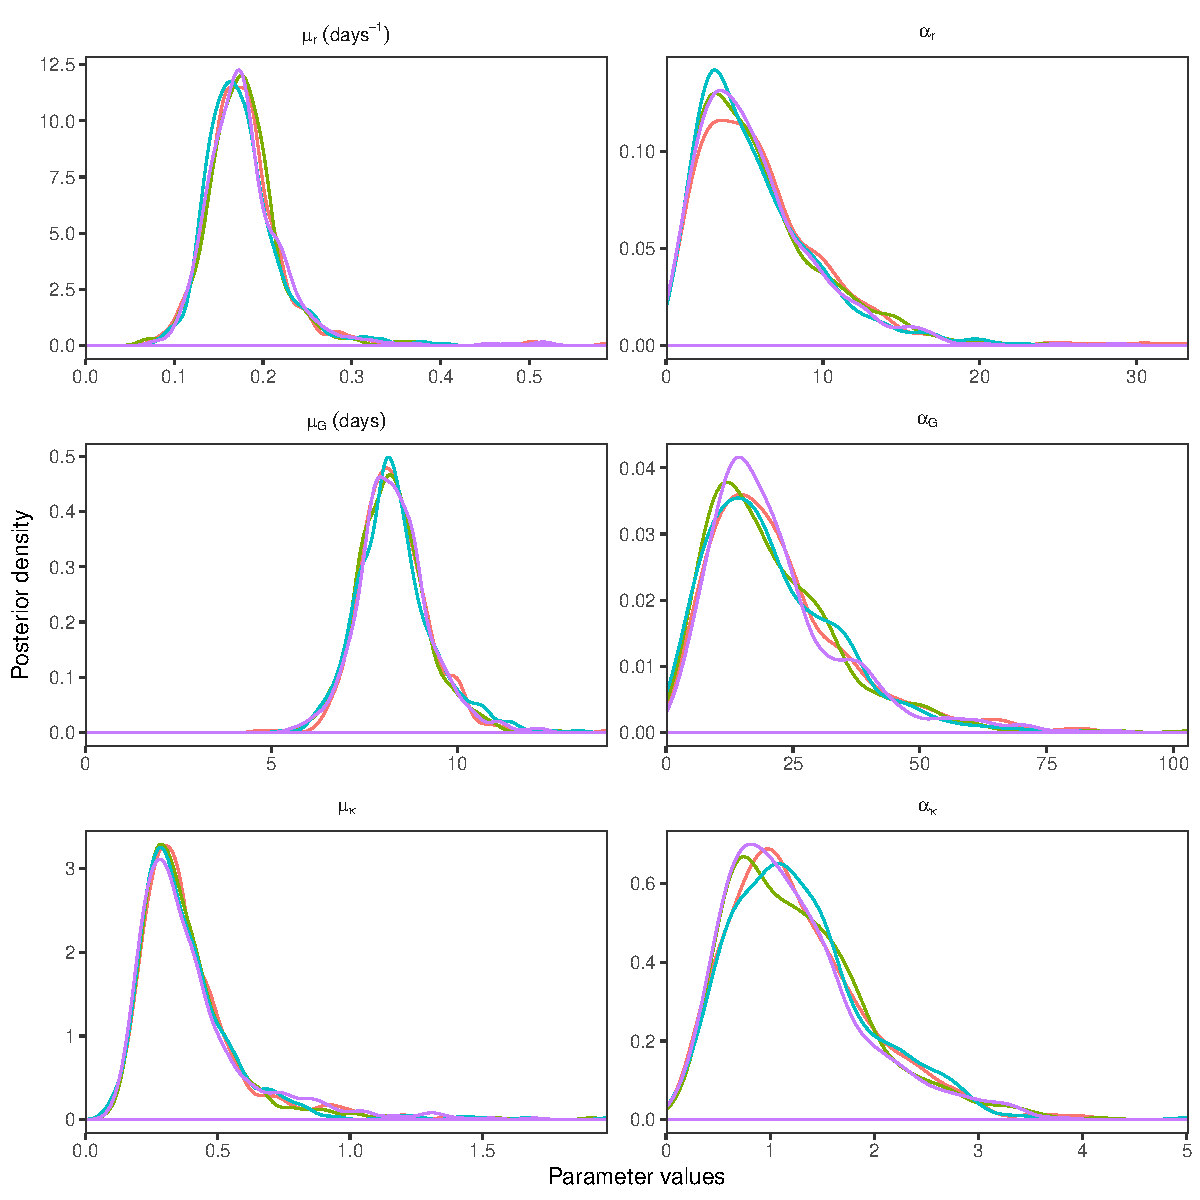
\includegraphics[width=\textwidth]{posterior_dist.pdf}
\caption{
\textbf{Marginal posterior distributions of the multilevel model.}
Each chain is represented by a different color.
}
\end{figure}

\end{document}
